\chapter{The CMS experiment at LHC}\label{chap:LHC_CMS}
This chapter introduces the Compact Muon Solenoid (CMS) experiment at the Large Hadron Collider (LHC). The description of CMS detector is presented starting form the innermost region to the outermost one. Before that, a short introduction to the LHC is given including the design of the LHC as well as the phenomenology of the proton-proton interactions.
\section{The Large Hadron Collider (LHC)}\label{sec:LHC}
The Large Hadron Collider (LHC) is the world's largest and most powerful particle accelerator. It was built by the European Organization for Nuclear Research (CERN) between 1998 and 2008 in collaboration with over 10,000 scientists and engineers from over 100 countries, as well as hundreds of universities and laboratories. It has 26.7 kilometres circumference and is as deep as 175 meters beneath the France-Switzerland border near Geneva shown in left plot of Figure \ref{fig:LHC} and it first started up on 10 September 2008. There are four main experiments at LHC which are shown in right plot of Figure \ref{fig:LHC}, the general description about the four experiments are in the following:
\begin{enumerate}
\item $\mathbf{ALTAS:}$ One of two general-purpose detectors. ATLAS investigates many different types of physics that might become detectable in the energetic collisions of the LHC. Some of these are confirmations or improved measurements of the SM (like study the Higgs boson and top quark), while many others are possible clues for new physical theories (like supersymmetry, extra dimensions, and microscopic black holes theories).
\item $\mathbf{CMS:}$ The other general-purpose detector, like ATLAS, studies the SM and looks for clues of new physics. The CMS detector is described in Section \ref{sec:CMS}.
\item $\mathbf{ALICE:}$ ALICE is optimized to study heavy-ion (Pb-Pb nuclei) collisions and is focusing on the physics of strongly interacting matter at extreme energy densities.
ALICE is studying a  ``fluid'' form of matter called quark-gluon plasma which are believed to have existed a fraction of the second after the Big Bang before quarks and gluons bound together to form hadrons and heavier particles and its properties are key issues in QCD physics.
\item $\mathbf{LHCb:}$ The experiment has wide physics program covering many important aspects of heavy flavor (both beauty and charm), electroweak, and QCD physics. Like measuring the parameters of CP violation in the interactions of b-hadrons (hadrons containing a bottom quark) and such studies can help to explain the matter-antimatter asymmetry of the Universe. The detector is also able to perform measurements of production cross sections and electroweak physics in the forward region.
\end{enumerate}

\begin{figure}[h!]
\begin{center}
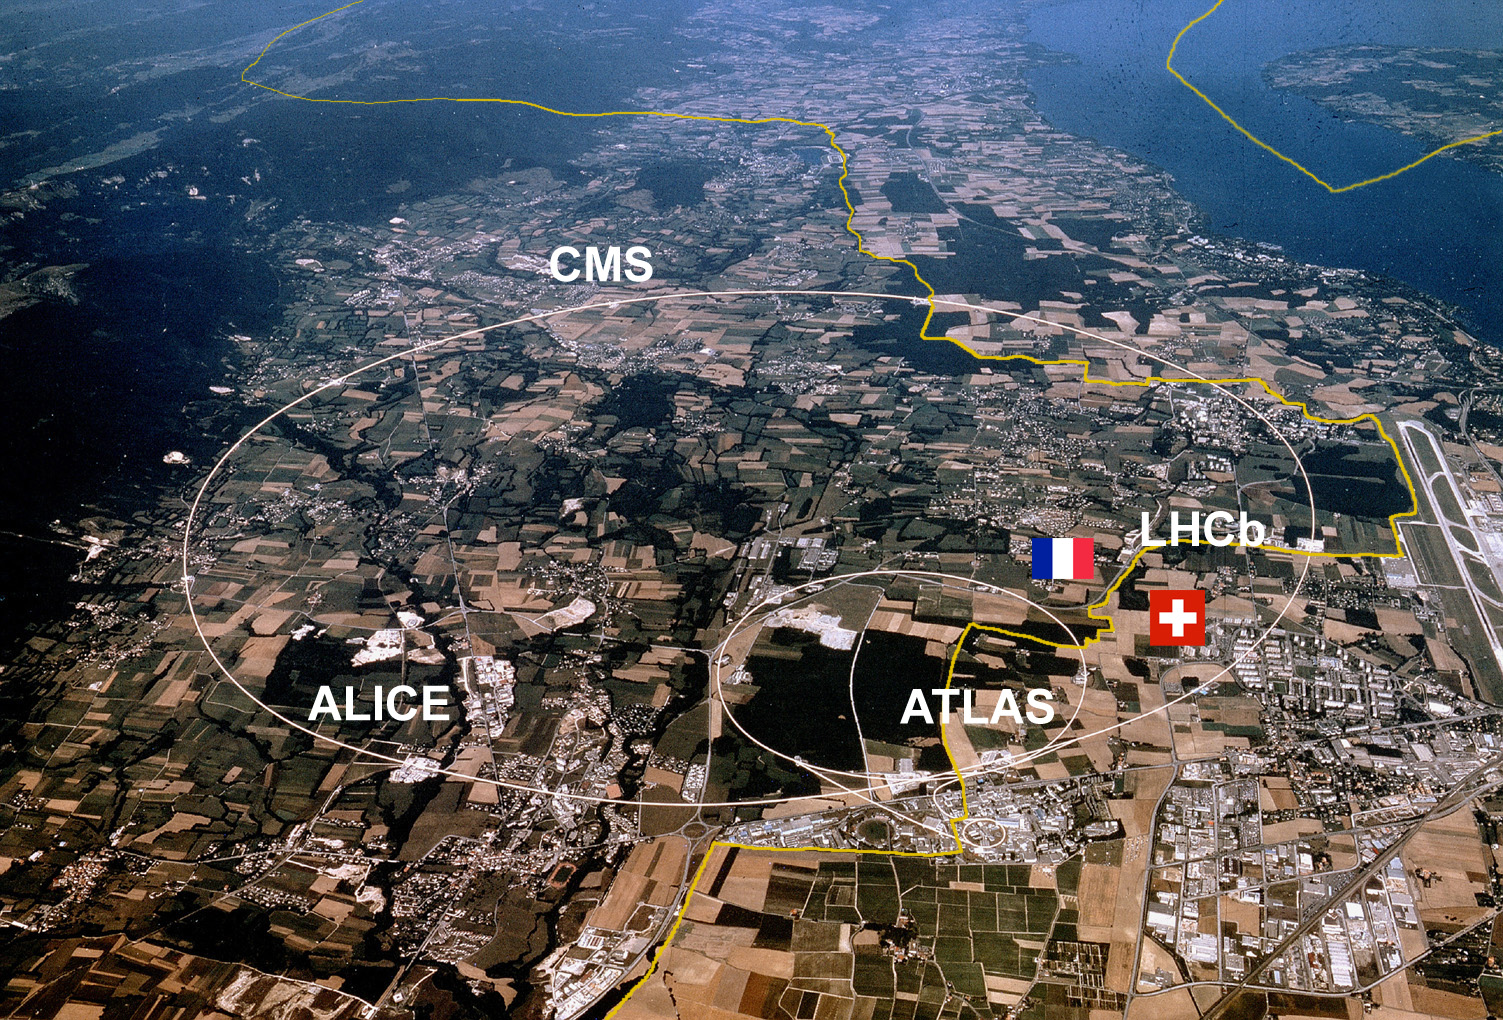
\includegraphics[width=0.49\textwidth]{figures/LHC/LHC.jpeg}
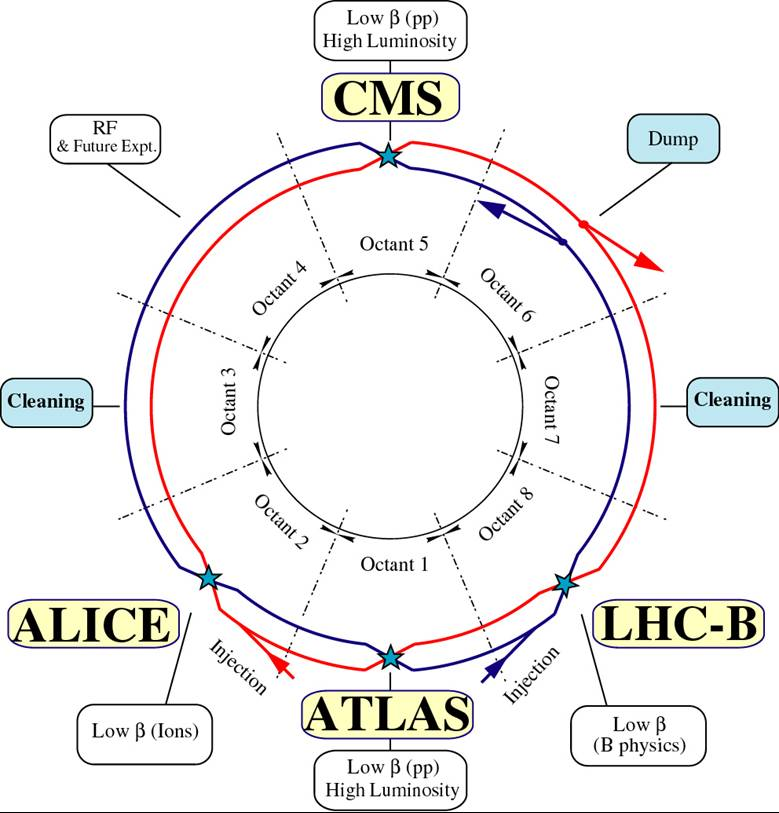
\includegraphics[width=0.49\textwidth]{figures/LHC/LHC2.jpg}
\caption{The overview of LHC (left) and the four main experiments in LHC (right) \cite{LHC_FourExp}.}
\label{fig:LHC}
\end{center}
\end{figure}

\subsection{Proton proton collision}\label{sec:LHC_pp_collision}
The reason to choose proton as accelerating particle in the LHC is that proton is stable, easy to get and has very low synchrotron radiation comparing to the electron, so it can be accelerated to very high energy. The reason for choosing colliding beams is that it gives much higher effective collision energy (or the centre of mass energy $E_{cm}$) which is shown in equation \ref{eq:Colliding_Ecm} assuming $\bf{p_{1}}$ is the four-vector $\mathbf{p}=(E,\overrightarrow{p})$ for proton 1 and $\mathbf{p_{2}}$ is the four-vector for proton 2. For example when two 7 TeV protons collide, the $E_{cm}$ is 14 TeV, but if one of the two protons is at rest, the $E_{cm}$ is 114.6 GeV.
\begin{equation}
\begin{split}
&E_{cm}^{2}=(\mathbf{p_{1}}+\mathbf{p_{2}})^{2}=(E_{1}+E_{2})^{2}-(\overrightarrow{p_{1}}+\overrightarrow{p_{2}})^{2}, \\
&E_{cm}^{2}=(E_{1}+E_{2})^{2} \mathrm{~when~proton~1~and~proton~2~collide},                                  \\
&E_{cm}^{2}=(m_{1}^{2}+m_{2}^{2}+2m_{2}E_{1,lab}) \mathrm{~when~proton~2~is~at~rest}.                          \\
\end{split}
\label{eq:Colliding_Ecm}
\end{equation}

The LHC acceleration chain for the protons is shown in Figure \ref{fig:LHC_chain}. At first the linear particle accelerator LINAC 2 generates 50 MeV protons, which feeds the Proton Synchrotron Booster (PSB). In the PSB the protons are accelerated to 1.4 GeV and injected into the Proton Synchrotron (PS), where they are accelerated to 26 GeV and the proton bunches are formed with the correct 25 ns spacing. Then the proton beam is subsequently accelerated to 450 GeV in the Super Proton Synchrotron (SPS) and transferred to the LHC main ring. In the main ring the proton beam is accelerated in two adjacent parallel beam pipes with opposite travel direction and until they reach the target energy. Finally the proton proton collision occur at the points of the main experiments (shown in right plot of Figure \ref{fig:LHC}).
\begin{figure}[h!]
\begin{center}
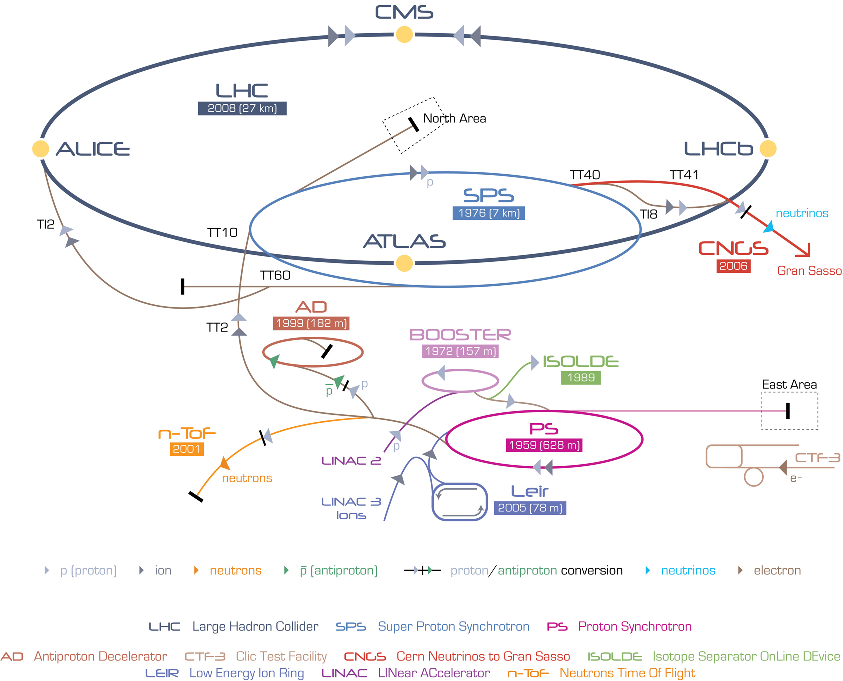
\includegraphics[width=0.99\textwidth]{figures/LHC/lhc_accelerator_chain.png}
\caption{The overview of LHC accelerator chain \cite{CERN_WEB}.}
\label{fig:LHC_chain}
\end{center}
\end{figure}
\subsection{Pile up}\label{sec:LHC_pileup}
In the LHC the collisions are between proton bunches and there are $\mathcal{O}(10^{11})$ protons per bunch. Depending on the instantaneous luminosity of the beam (see next section), there may be several proton proton collisions in the same bunch crossing. This phenomenon is so-called pile up, and is shown in the left plot of Figure \ref{fig:LHC_pileup}. The pile up distributions for proton proton collisions in 2016 and 2017 are shown in the middle plot and right plot of Figure \ref{fig:LHC_pileup}.
\begin{figure}[h!]
\begin{center}
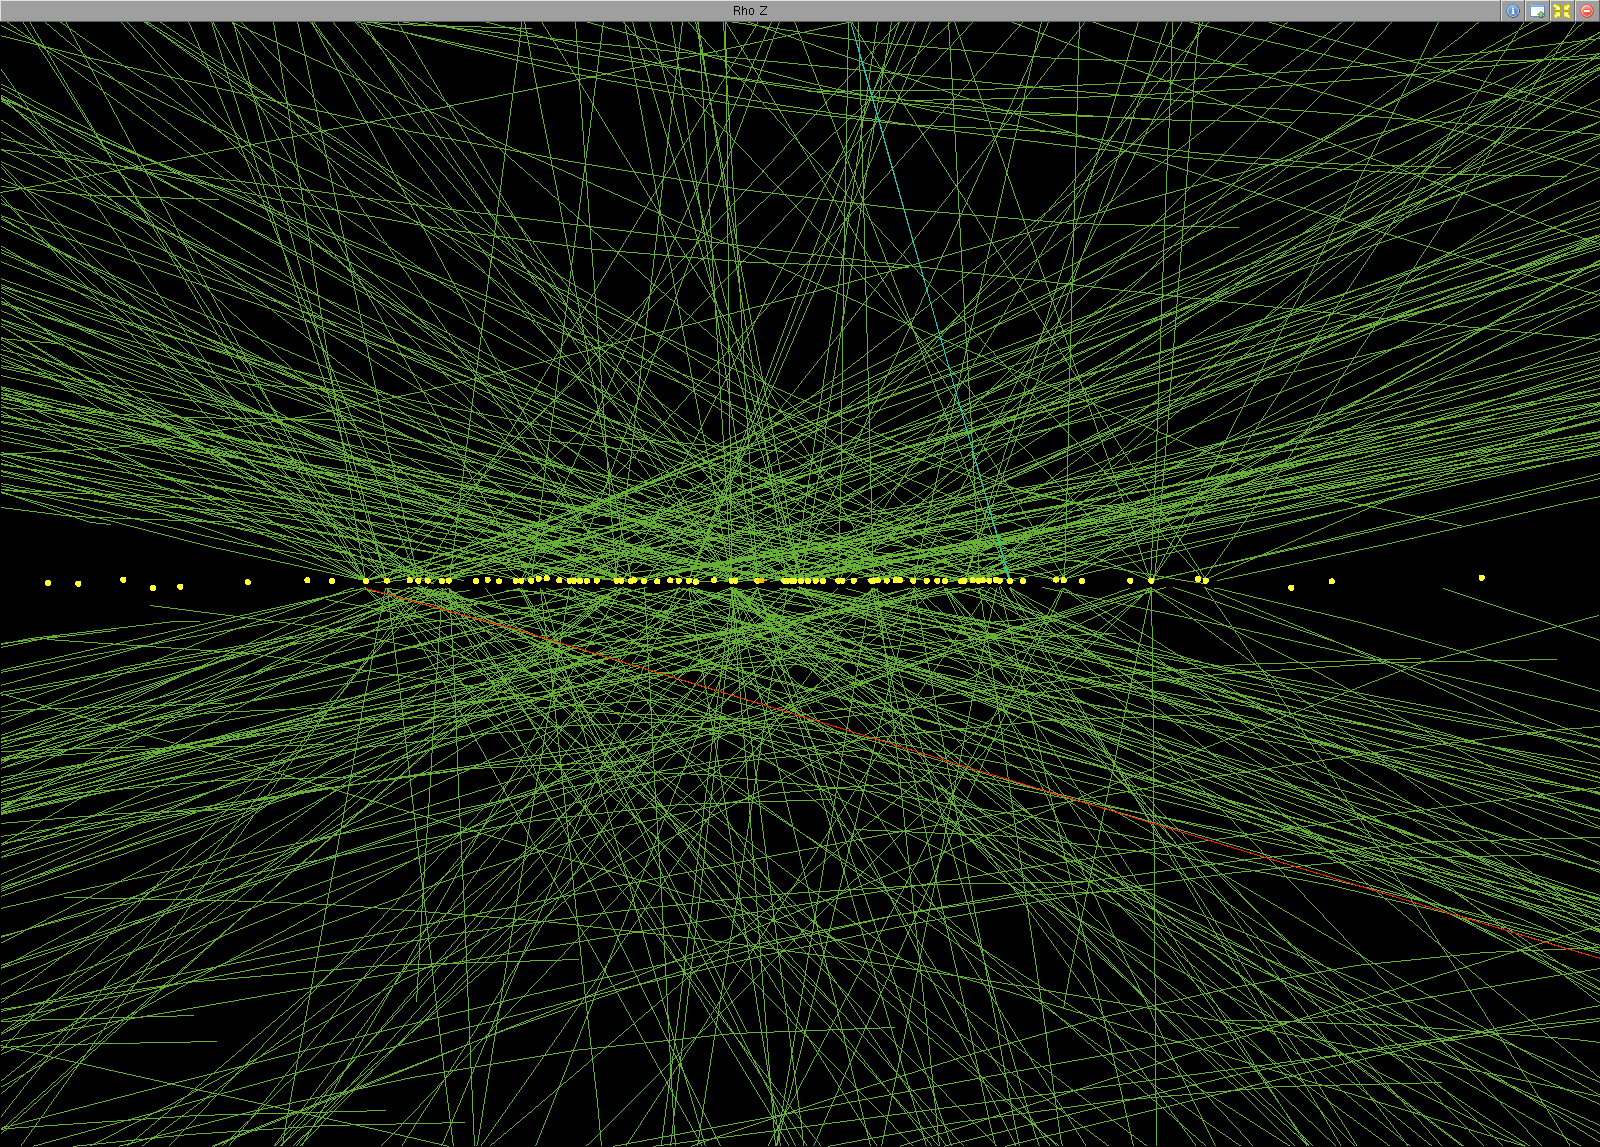
\includegraphics[width=0.32\textwidth]{figures/LHC/pile-up.png}
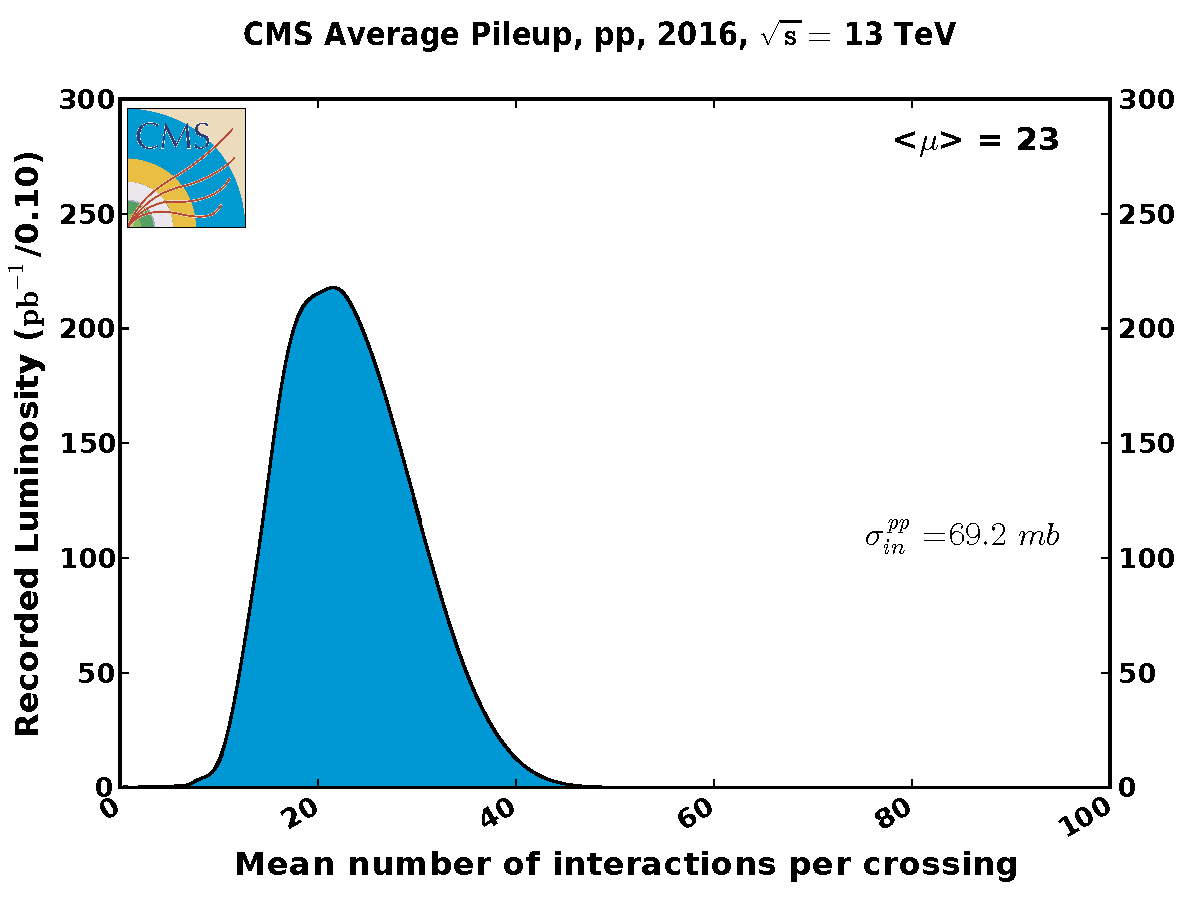
\includegraphics[width=0.32\textwidth]{figures/LHC/pileup_pp_2016_69200.pdf}
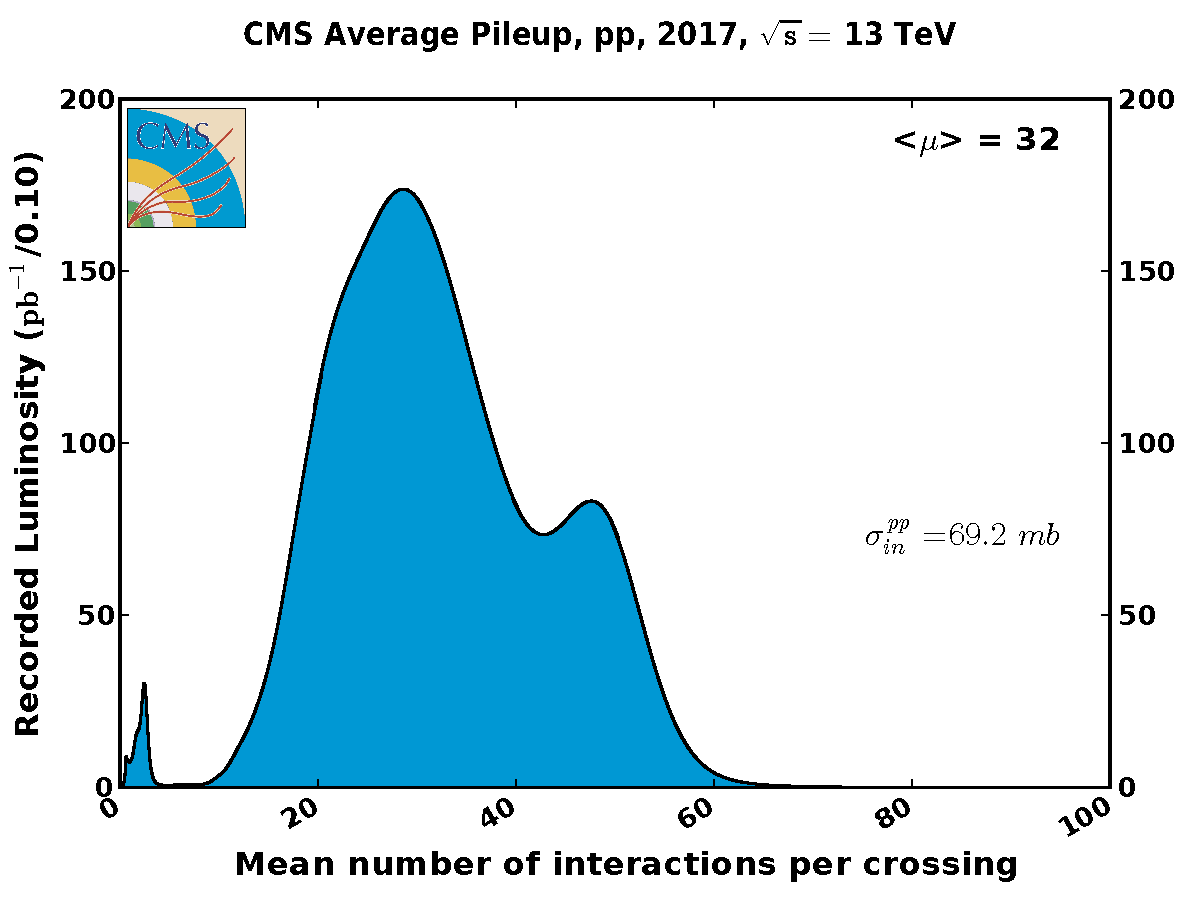
\includegraphics[width=0.32\textwidth]{figures/LHC/pileup_pp_2017_69200.pdf}
\caption{The phenomenon of pile up (left), the number of interaction per bunch crossing for 2016 (middle) and 2017 (right) \cite{CMS_Luminosity}.}
\label{fig:LHC_pileup}
\end{center}
\end{figure}
\subsection{Luminosity}\label{sec:LHC_luminosity}
The instantaneous luminosity ($\mathcal{L}$) is the proportionality factor
between the number of events detected per second (dN/dt) and the interaction cross section ($\sigma_{p}$):
\begin{equation}
\frac{dN}{dt}=\mathcal{L}\cdot\sigma_{p}
\label{eq:define_Lumi}
\end{equation}
The unit of the instantaneous luminosity is $\mathrm{cm^{-2}s^{-1}}$.
The instantaneous luminosity of two beams colliding head-on can be calculated by formula (\ref{eq:Lumi}) \cite{Herr2013}, where $N_{1}$ and $N_{2}$ are the numbers of particles per bunch in the beam 1 and in the beam 2, $N_{b}$ is the number of bunches in one beam, $f$ is the beam revolution frequency, and $\sigma_{x}$ and $\sigma_{y}$ are the 1 $\sigma$ gaussian widths of the bunch in the x axis and in the y axis directions, respectively (here the beam moving direction is along the z axis).
\begin{equation}
\mathcal{L}=\frac{N_{1}N_{2}N_{b}f}{4\pi\sigma_{x}\sigma_{y}}
\label{eq:Lumi}
\end{equation}

After integrating the instantaneous luminosity over time it gives so-called integrated luminosity:
\begin{equation}
\mathcal{L}_{int}=\int_{0}^{T}\mathcal{L}(t)dt
\label{eq:Integrated_Lumi}
\end{equation}
The cumulative online integrated luminosity that the LHC delivered and the one that CMS recorded for 2016 and 2017 are shown in Figure \ref{fig:LHC_luminosity}.
\begin{figure}[h!]
\begin{center}
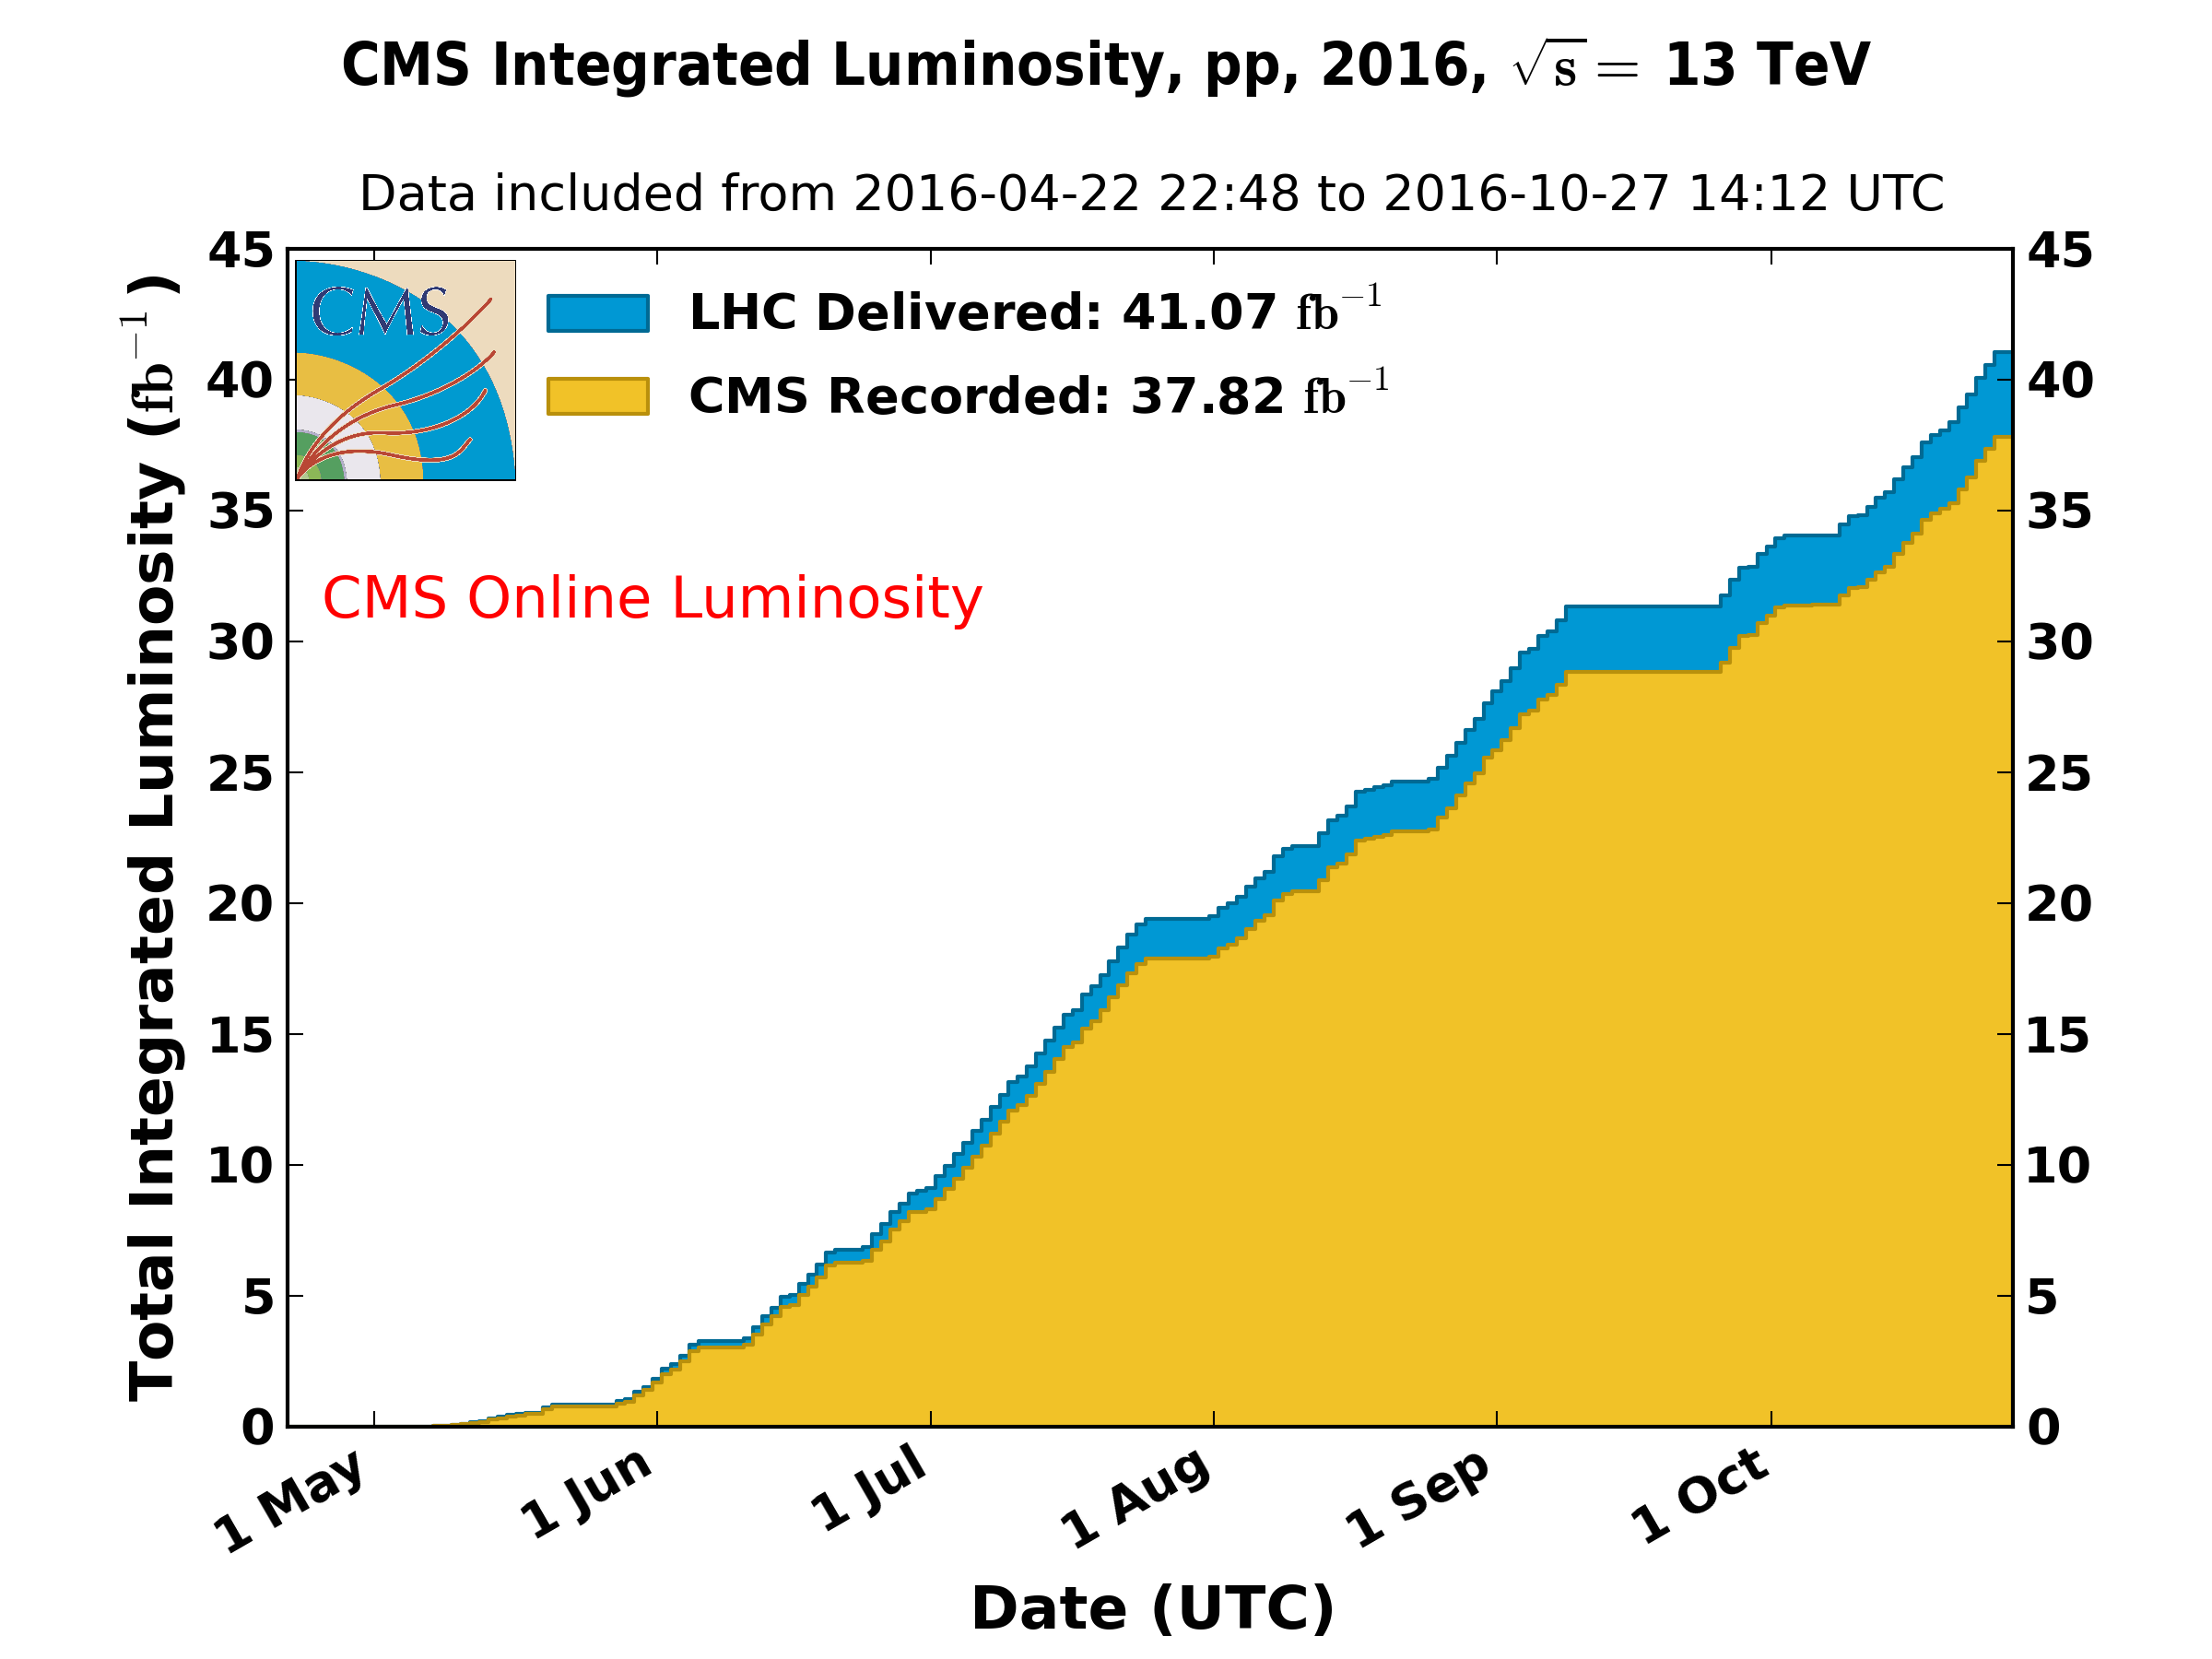
\includegraphics[width=0.49\textwidth]{figures/LHC/int_lumi_per_day_cumulative_pp_2016OnlineLumi.png}
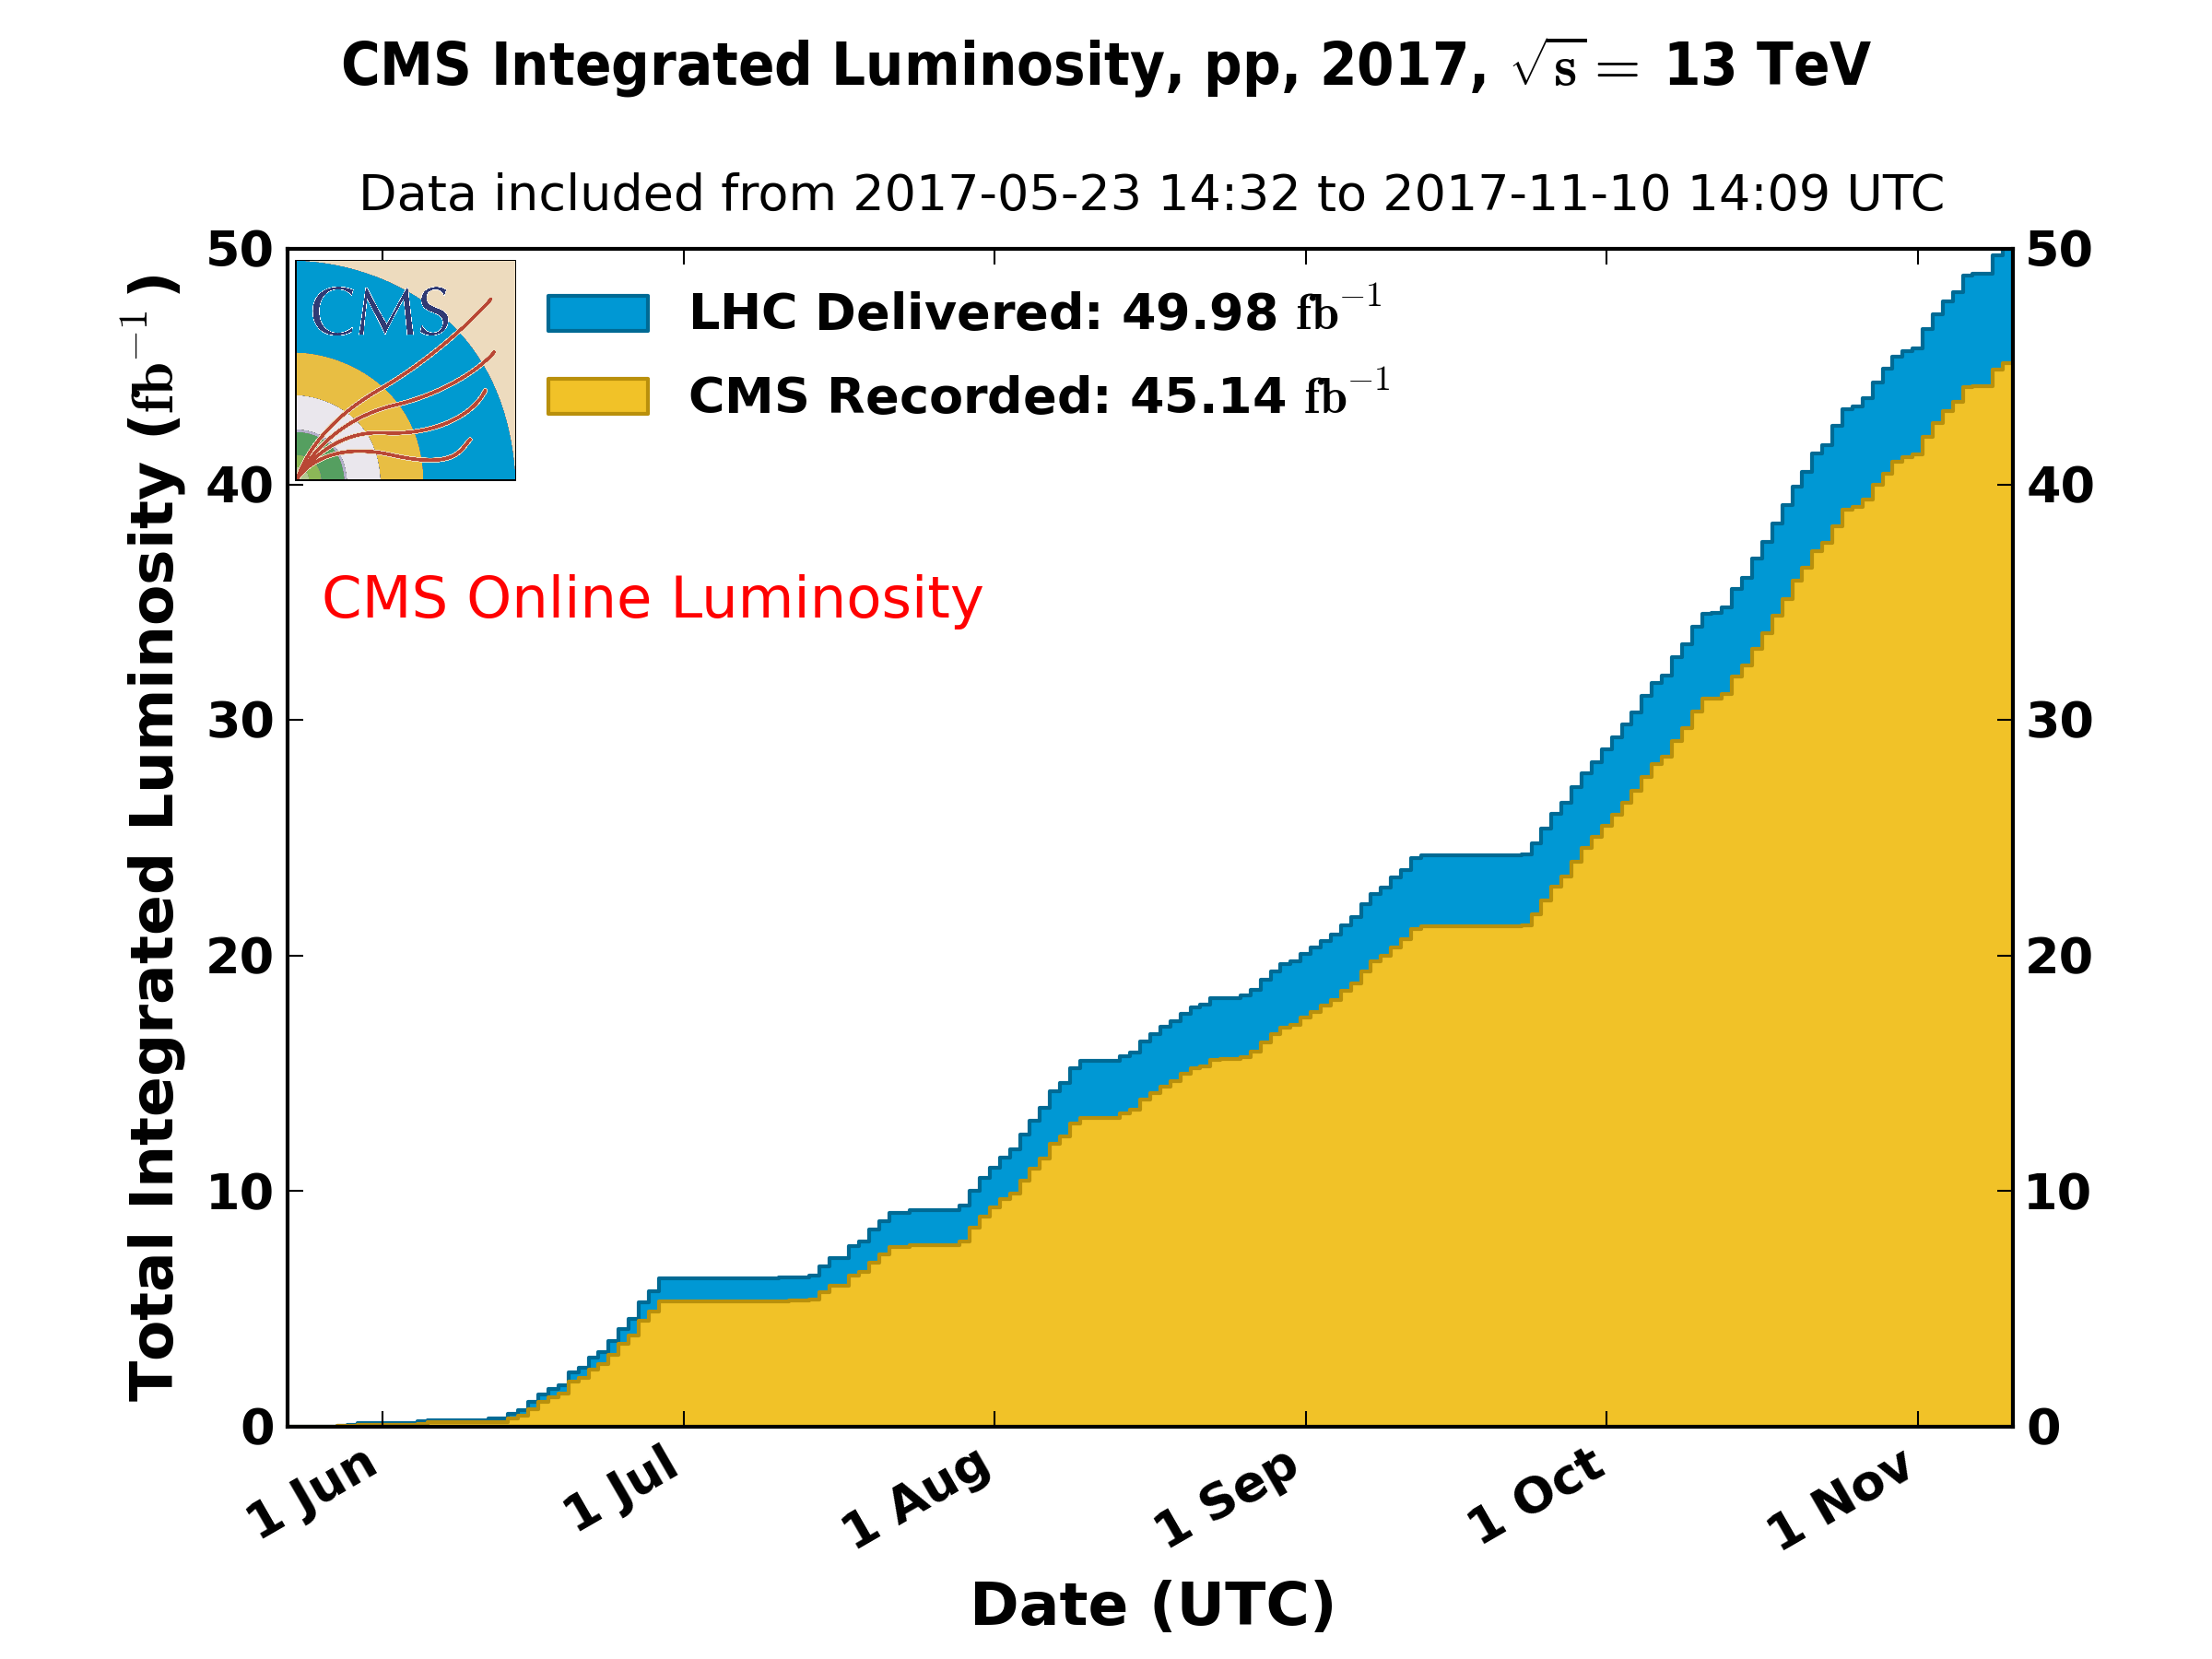
\includegraphics[width=0.49\textwidth]{figures/LHC/int_lumi_per_day_cumulative_pp_2017OnlineLumi.png}
\caption{The cumulative online integrated luminosities that the LHC delivered and the one that CMS recorded for 2016 (left) and 2017 (right) \cite{CMS_Luminosity}.}
\label{fig:LHC_luminosity}
\end{center}
\end{figure}

The plan of data taking of the LHC and for the High Luminosity LHC (HL-LHC) phase are shown in Figure \ref{fig:LHC_plan}. For Run 2 (from years 2015 to 2018), LHC has delivered 156 \fbinv data which is more than the planned data which is 150 \fbinv data. The LHC data taking conditions from its start-up in 2010 to 2018 are shown in Table \ref{tab:LHC_Lumi}. For HL-LHC the goal is to deliver 3000 \fbinv which is a factor of 10 increased compared with 300 \fbinv data which is the total luminosity expected to be delivered by the LHC at the end of Run 3 in 2023.



\begin{table}[!hbpt]
\begin{center}
\begin{tabular}{|c|c|c|c|c|c|}
\hline
                       & year & $\sqrt{s}$ & $\mathcal{L}_{int}$ & bunch spacing & pile up \\ \hline
\multirow{3}{*}{Run 1} & 2010 & 7 TeV  & 44.96 \pbinv  & 50 ns         & -       \\ \cline{2-6}
                       & 2011 & 7 TeV  & 6.10  \fbinv  & 50 ns         & 10      \\ \cline{2-6}
                       & 2012 & 8 TeV  & 23.30 \fbinv  & 50 ns         & 21      \\ \hline
\multirow{4}{*}{Run 2} & 2015 & 13 TeV & 4.21  \fbinv  & 25 ns         & 12      \\ \cline{2-6}
                       & 2016 & 13 TeV & 40.99 \fbinv  & 25 ns         & 23      \\ \cline{2-6}
                       & 2017 & 13 TeV & 49.79 \fbinv  & 25 ns         & 33      \\ \cline{2-6}
                       & 2018 & 13 TeV & 67.86 \fbinv  & 25 ns         & 32      \\ \hline

\end{tabular}
\end{center}
\caption{The LHC data taking conditions from its start-up in 2010 to 2018.}
\label{tab:LHC_Lumi}
\end{table}

\begin{figure}[h!]
\begin{center}
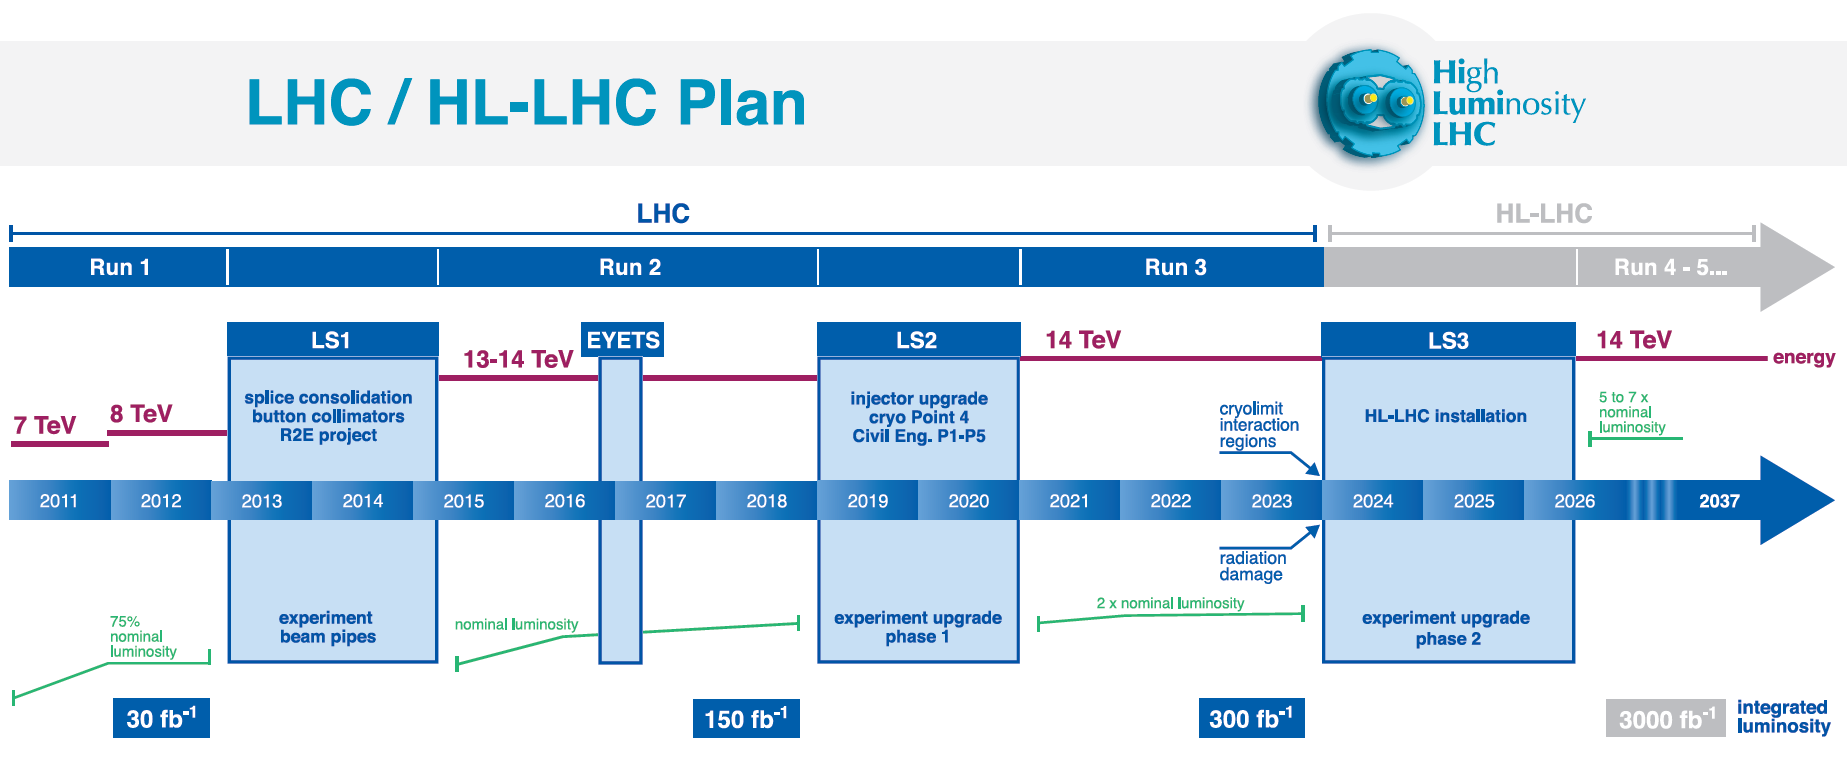
\includegraphics[width=0.9\textwidth]{figures/LHC/HL_LHC_PlanUpdateJuly2015.PNG}
\caption{The data delivery plan of LHC and HL-LHC \cite{Antonella:1975962}.}
\label{fig:LHC_plan}
\end{center}
\end{figure}


\section{The Compact Muon Solenoid (CMS)}\label{sec:CMS}
The Compact Muon Solenoid (CMS) is a general-purpose detector at the LHC. It has a broad physics programme ranging from studying the SM to searching for new physics. The CMS detector is built around a huge solenoid magnet. It is a cylindrical coil of superconducting cables that generates a field of 3.8 Tesla (T) and the field is confined by a steel  ``yoke'' which has a 14,000-tonne weight. The complete detector is 21 meters long, 15 meters wide, and 15 meters high. A one-quarter cross-sectional view of the CMS detector is shown in Figure \ref{fig:CMS_overview} together with some labels used to name the
detector elements. The transversal view of the CMS detector is shown in Figure \ref{fig:CMS_transversal}, together with the effect of the various sub-detectors response to the different incoming particles. The different elements of the CMS detector from the innermost to the outermost are:

\begin{enumerate}
\item $\mathbf{Inner~tracking~system}$ which measures the trajectory of charged particles and reconstructs secondary vertices;
\item $\mathbf{Electromagnetic~calorimeter}$ which measures the energy of electrons and photons;
\item $\mathbf{Hadronic~calorimeter}$ which measures the energy of hadrons;
\item $\mathbf{Superconducting~magnet}$ which provides a 3.8 T magnetic field parallel to the beam axis to bend the tracks of charged particles;
\item $\mathbf{Muon~system}$ which identifies and measures the trajectories of muons.
\end{enumerate}
In addition, because of the high collision rate at the LHC, a trigger system has been designed to only record data that is interesting for physics analyses.

\begin{figure}[h!]
\begin{center}
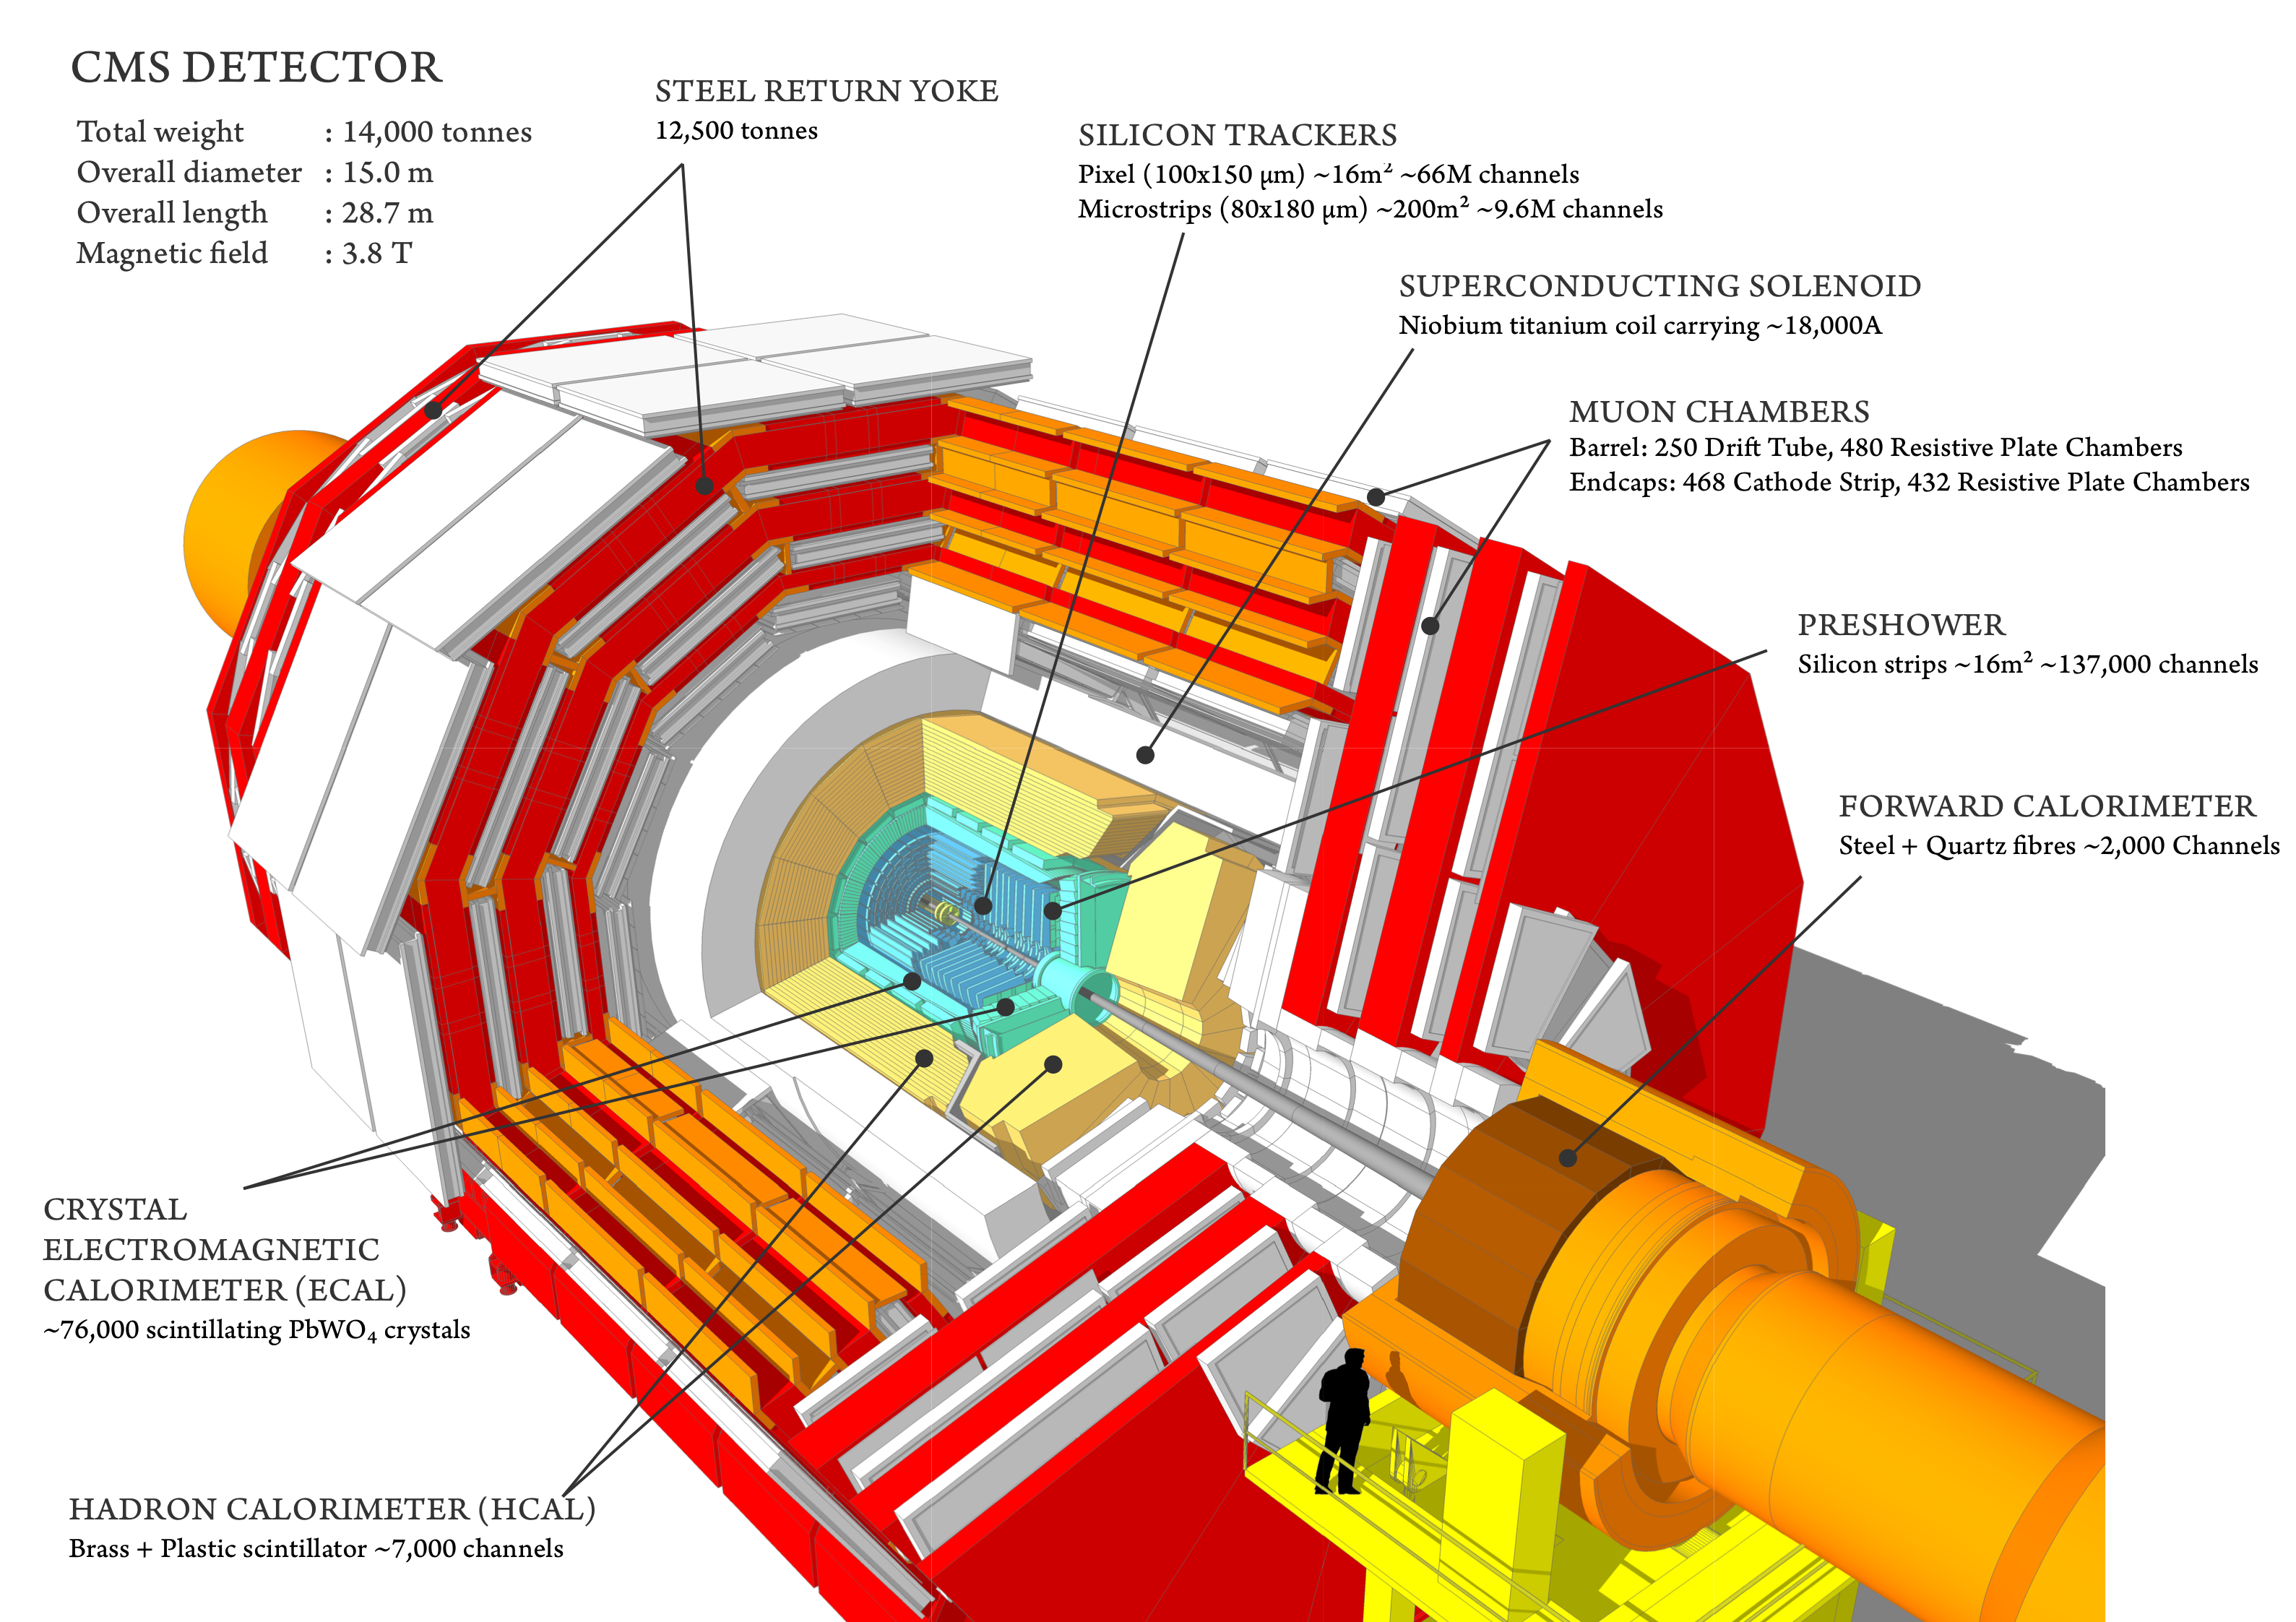
\includegraphics[width=0.9\textwidth]{figures/CMS/cms.png}
\caption{The exploded view of the CMS detector \cite{CMS_Detector1}.}
\label{fig:CMS_overview}
\end{center}
\end{figure}

\begin{figure}[h!]
\begin{center}
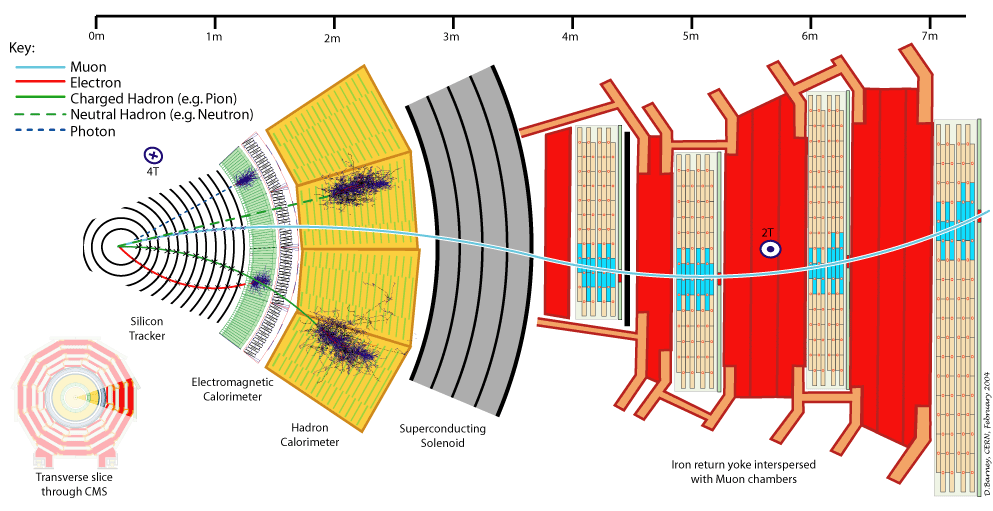
\includegraphics[width=0.9\textwidth]{figures/CMS/cms_particles.png}
\caption{The transversal view of the CMS detector \cite{CMS_Detector2}.}
\label{fig:CMS_transversal}
\end{center}
\end{figure}



Before moving to a detailed description of the CMS subdectors, the coordinate convention is described in the following section.
\subsection{Coordinate conventions}\label{subsec:CMS_Coordinate}

The coordinate system adopted by CMS has the origin centered at the nominal collision point inside the experiment, the y-axis pointing vertically upward, and the x-axis pointing radially inward toward the center of the LHC. Thus, the z-axis points along the beam direction toward the Jura mountains. The azimuthal angle $\phi$ is measured from the
x-axis in the x-y plane. The polar angle $\theta$ is measured from the z-axis. The coordinate system is shown in Figure \ref{fig:CMS_coordinate}. Pseudorapidity is defined as $\eta=-\mathrm{ln~tan}(\theta/2)$. The momentum of a particle measured transverse to the beam direction and in the beam direction, denoted by \pt and \pZ, respectively, are: $\mathrm{\pt=psin\theta}$ and $\mathrm{p_{Z}=pcos\theta}$, where p is the magnitude of the 3-momentum of the particle p = $|\overrightarrow{p}|$.
%The imbalance of energy measured in the transverse plane is denoted by $\et^{miss}$ (or $\cancel{E}_T$) which is computed by $\overrightarrow{\et^{miss}}=-\sum\overrightarrow{\et^{exists}}$ (more details in Section \ref{sec:MET}).

\begin{figure}[h!]
\begin{center}
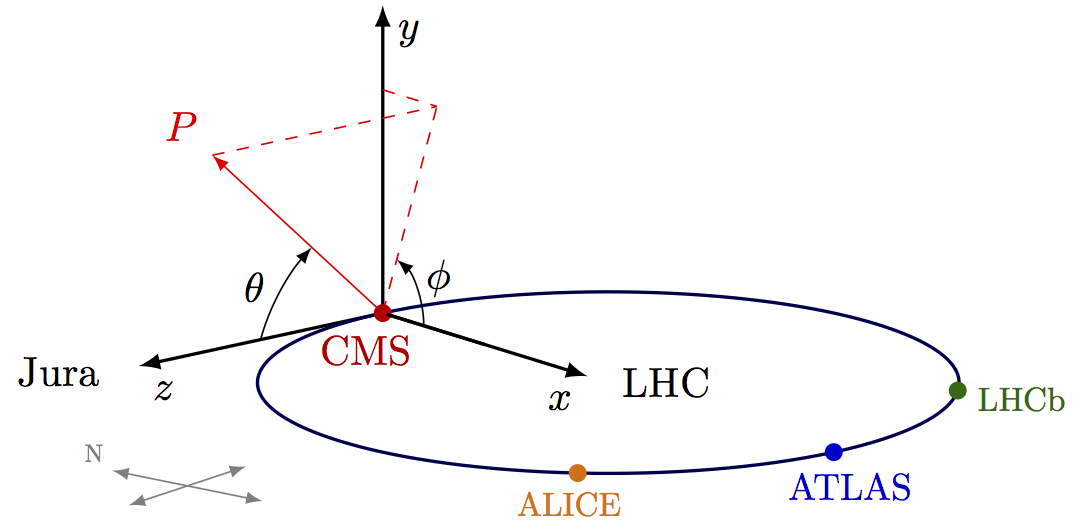
\includegraphics[width=0.5\textwidth]{figures/CMS/cms_coordinate_system.png}
\caption{The CMS coordinate system.}
\label{fig:CMS_coordinate}
\end{center}
\end{figure}
\subsection{Tracking system}\label{subsec:CMS_tracker}


The CMS tracking system is used for reconstructing the trajectories of charged particle. The tracker system is composed of two sub-detectors immersed in a 3.8 T magnetic field produced by an external solenoidal magnet (detailed in Section \ref{subsec:CMS_Magnet}). Referring to Figure \ref{fig:CMS_tracker}, the innermost detector, closest to the beam pipe, is the silicon pixel detector, while the outer detector is the silicon strip detector.

The silicon pixel detector is the innermost part of the CMS detector. It provides space point measurements of charged particle trajectories within a pseudorapidity up to $|\eta|=2.5$ . The pixel detector has been designed to withstand an instantaneous luminosity of $1\times10^{34}~\mathrm{cm^{-2}s^{-1}}$ with a bunch spacing of 25 ns. The pixel detector comprises three layers in the barrel (TPB) region and two endcap (TPE) disks at each side of the barrel which is shown in Figure \ref{fig:CMS_pixel_detector}. The three barrel layers are located at mean radii of 4.4 cm, 7.3 cm and 10.2 cm, and have a length of 53 cm. The two endcap disks, extending from 6 to 15 cm in radius, are placed on each side at $\mathrm{|z|}$ = 34.5 cm and 46.5 cm. In order to achieve the optimal vertex position resolution, the designed size of pixels is 100$\times$150 $\mu \mathrm{m^{2}}$. It has a sensitive area of 1.1 \mTwo and is segmented into 66 (48 in TPB and 18 in TPE) million pixels. The endcap disks are assembled in a turbine-like geometry with blades rotated by $20^{\circ}$ to
 benefit from the large Lorentz drift angle in the magnetic field. The measured hit resolution in the TPB is 9.4 $\upmu$m in the r-$\phi$ plane and 20-40 $\upmu$m in the longitudinal direction which depends on the angle of the track relative to the sensor.

It is worth mention that during Run 2 the instantaneous luminosity of LHC has significantly increased and it was around to $2\times10^{34}~\mathrm{cm^{-2}s^{-1}}$. The number of pileup events has then increased to 50 or more which, together with ongoing radiation damage, will potentially lead to a loss in tracking efficiency. To maintain the high tracking efficiency, the pixel detector was updated during an extended winter shutdown in 2016/2017.  The new detector (hereafter referred to as the Phase 1 pixel detector) consists of four layers in the barrel (BPIX), which represents an additional layer compared to the old detector. The radius of the innermost layer was reduced from 44 mm to 30 mm. In the endcap region (FPIX) a third disk was added per side. The new detector therefore allows a four-point coverage in the whole tracking region and the number of channels is almost double from 66 millions to 124 millions with keeping the same pixel size. A comparison of the old and new designs is shown in Figure \ref{fig:CMS_pixel_update}.

The silicon strip tracker is placed outside of the pixel tracker. It has 10 layers in the barrel region, four in the inner barrel (TIB), and 6 in the outer barrel (TOB). It also has two endcaps, each one made up of 3 inner disks (TID) and 9 outer disks (TEC). It is composed of 9.6 millions silicon strips with a pitch varying from 80 to 205 $\mu \mathrm{m}$. The total area of the Si detectors is around 200 \mTwo, providing a coverage up to $|\eta|$ = 2.5. In order to provide 3-dimensional information, several layers in the barrel and in the endcap have stereo modules with two silicon strip modules mounted back-to-back and rotated by 100 mrad with respect to each other.
This leads to a single point resolution between 23-34 $\upmu$m in the r-$\phi$ direction and 23 $\upmu$m in z direction for TIB, for TOB it is from 35-52 $\upmu$m in the r-$\phi$ direction and 52 $\upmu$m in z direction. The single point resolution that can be achieved depends strongly on the size of the cluster and on the pitch of the sensor and varies not only as a function of the cluster width, but also as a function of pseudorapidity, as the energy deposited by a charged particle in the silicon depends on the angle at which it crosses the sensor plane.
\begin{figure}[h!]
\begin{center}
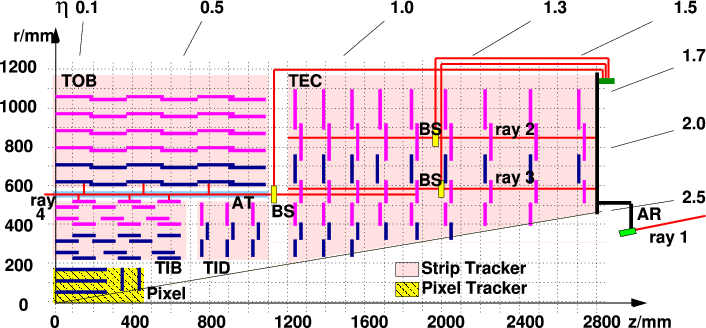
\includegraphics[width=0.8\textwidth]{figures/CMS/tracker/cms_tracker.png}
\caption{The tracker layout (1/4 of the z view) \cite{Chatrchyan:2008aa}.}
\label{fig:CMS_tracker}
\end{center}
\end{figure}

\begin{figure}[h!]
\begin{center}
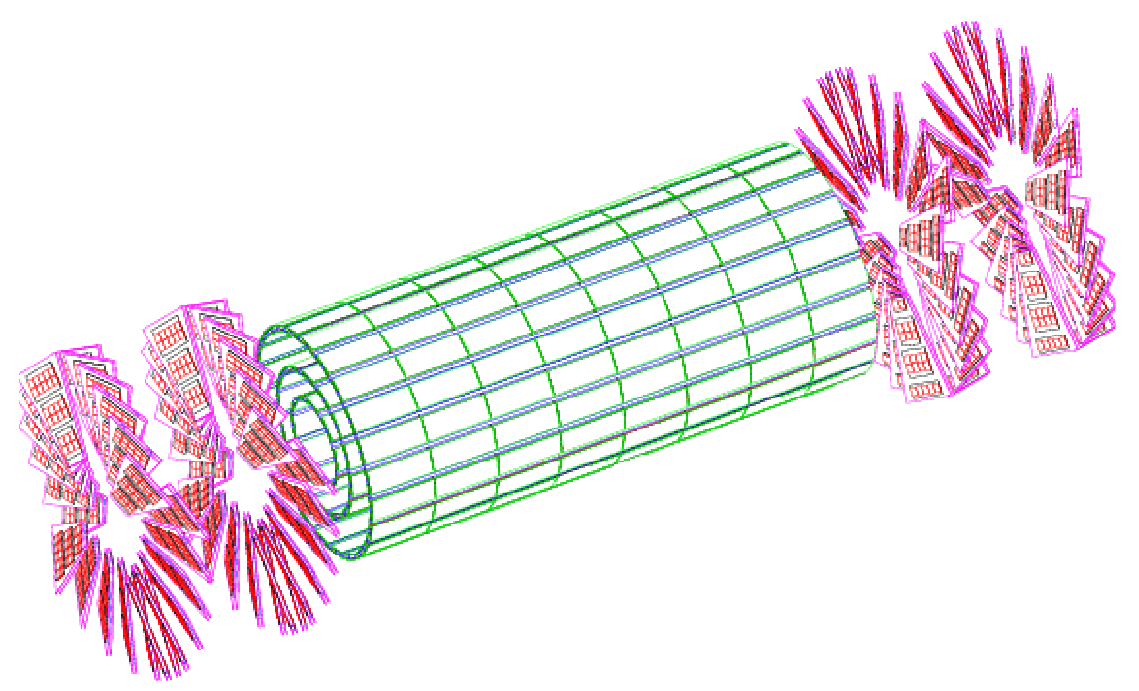
\includegraphics[width=0.8\textwidth]{figures/CMS/tracker/cms_pixelDetector.png}
\caption{Layout of pixel detectors in the CMS tracker \cite{Chatrchyan:2008aa}.}
\label{fig:CMS_pixel_detector}
\end{center}
\end{figure}

\begin{figure}[h!]
\begin{center}
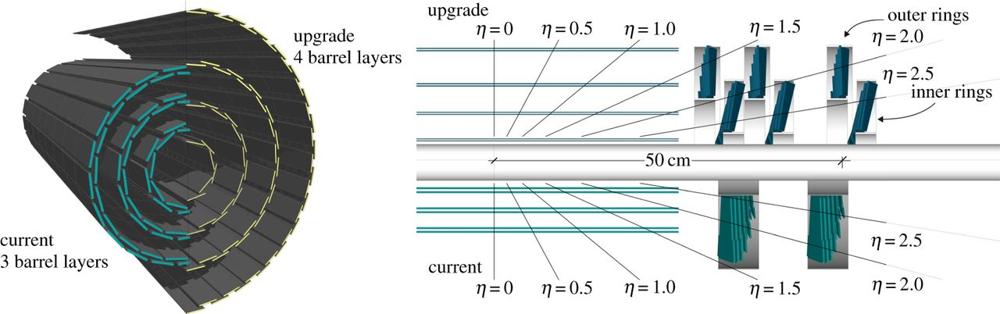
\includegraphics[width=0.8\textwidth]{figures/CMS/tracker/pixel_phase1_update.png}
\caption{Comparison of the Phase 1 pixel detector (above the beam pipe) and the 2016 detector layout (under the beam pipe) \cite{Chatrchyan:2008aa}.}
\label{fig:CMS_pixel_update}
\end{center}
\end{figure}

\subsection{Electromagnetic calorimeter}\label{subsec:CMS_ECAL}
In order to measure the energy of electrons and photons the CMS detector uses electromagnetic calorimeter (ECAL), which is placed outside of the tracker system. The ECAL is a hermetic, homogeneous calorimeter comprising 61200 lead tungstate (\PbWO) crystals mounted in the central barrel part, closed by 7324 crystals in each of the 2 endcaps with coverage in pseudorapidity up to $|\eta| < 3.0$. A preshower system is installed in front of the edges of ECAL endcap for \pizero rejection. A 3D view of the barrel and endcap electromagnetic calorimeter is shown in Figure \ref{fig:CMS_Ecal_1}. The reason to choose lead tungstate scintillating crystals for ECAL is because it has short radiation length ($X_{0}$ = 0.89 cm, for electron, the radiation lengths is the mean distance over which the electron loses all but 1/e of its energy by bremsstrahlung.) and Moliere radius (2.2 cm, Moliere radius is the radius of a cylinder containing on average 90\% of the shower's energy deposition.).
Besides, its radiation is fast (80\% of the light is emitted within 25 ns) and hard (up to 10 mrad). However, the relatively low light yield (30 $\gamma$/MeV) requires use of photodetectors with intrinsic gain that can operate in a magnetic field. Silicon avalanche photodiodes (APDs) are used as photodetectors in the barrel and
vacuum phototriodes (VPTs) in the endcaps. In addition, the sensitivity of both the crystals and the APD response to temperature changes requires a temperature stability (the goal is
$0.1^{\circ}$ C). The use of \PbWO crystals has thus allowed the design of a compact calorimeter inside the solenoid that is fast, has fine granularity, and is radiation resistant.


\begin{figure}[h!]
\begin{center}
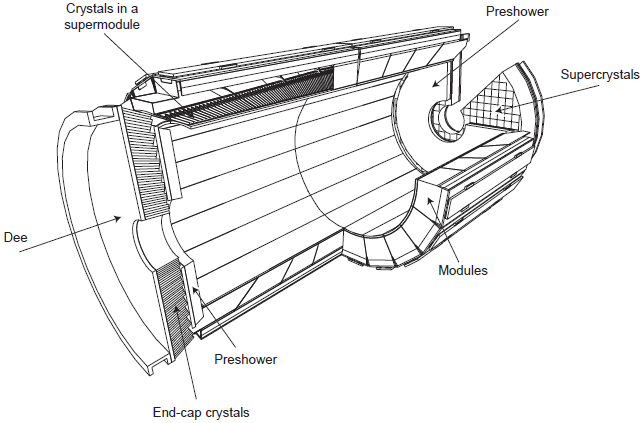
\includegraphics[width=0.8\textwidth]{figures/CMS/ECAL/ECAL.png}
\caption{A 3D view of the barrel and endcap electromagnetic calorimeter \cite{Chatrchyan:2008aa}.}
\label{fig:CMS_Ecal_1}
\end{center}
\end{figure}

The barrel part of the ECAL covers the pseudorapidity range $|\eta|$ < 1.479 (see Figure \ref{fig:CMS_Ecal_2}). The front face of the crystals is at a radius of 1.29 m and each crystal has a square cross-section of $\approx$ 22$\times$22 \mmTwo and a length of 230 mm corresponding to 25.8 $X_{0}$. The truncated pyramid-shaped crystals are mounted in a geometry which is off-pointing with respect to the mean position of the primary interaction vertex, with a $3^{\circ}$ tilt in both $\phi$ and in $\eta$, in order to avoid the scenario in which a particle could go right along the separation between two center-pointing crystals. The crystal cross-section corresponds to $\Delta\eta\times\Delta\phi=0.0175\times0.0175~(1^{\circ})$. The barrel granularity is 360-fold in $\phi$ and 2$\times$85-fold in $\eta$, resulting in a total number of 61200 crystals. The crystal volume in the barrel amounts to 8.14 \mThree (67.4 t). Crystals for each half-barrel are grouped in 18 supermodules each subtending $20^{\circ}$ in
$\phi$. Each supermodule comprises four modules with 500 crystals in the first module and 400 crystals in each of the remaining three modules (see Figure \ref{fig:CMS_Ecal_Barrel_supermodule}). For simplicity of construction and assembly, crystals are grouped in arrays of 2$\times$5 crystals which are contained in a very thin wall (200 $\upmu$m) alveolar structure and form a submodule.

\begin{figure}[h!]
\begin{center}
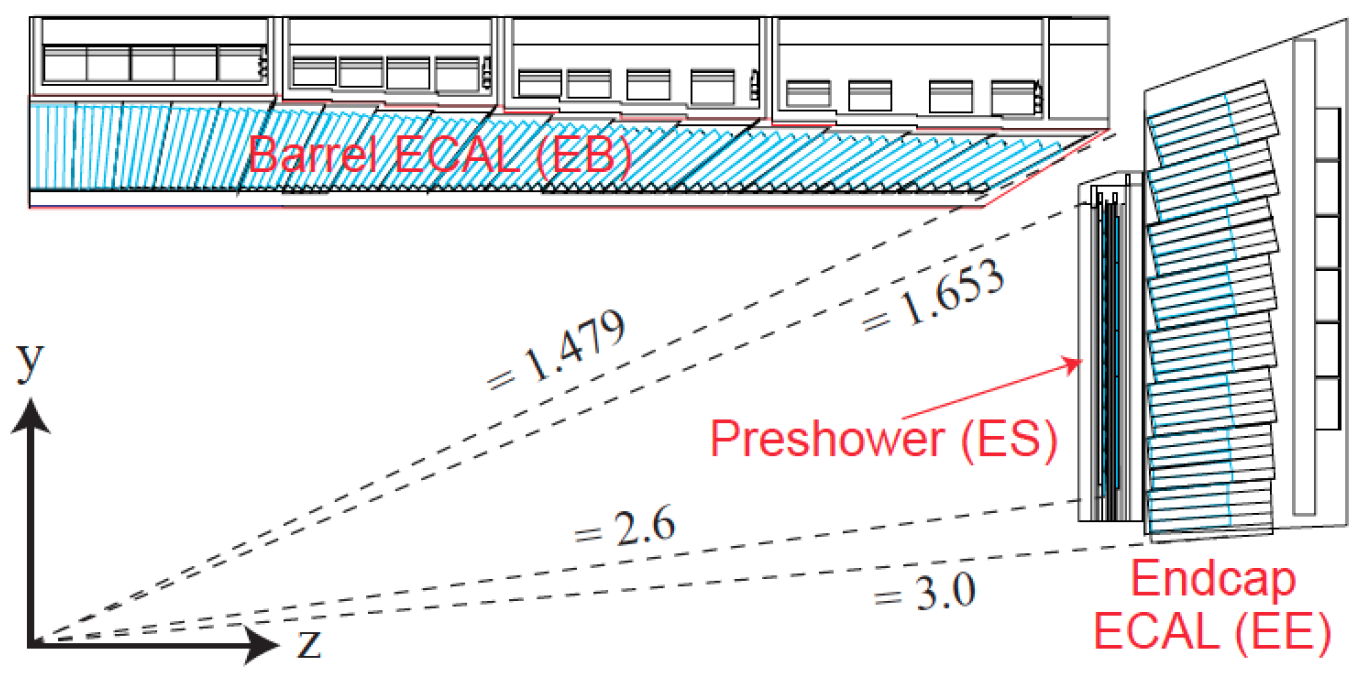
\includegraphics[width=0.8\textwidth]{figures/CMS/ECAL/Ecal_layout.png}
\caption{Longitudinal view of the electromagnetic calorimeter (one quadrant) \cite{CMS_TDR1}.}
\label{fig:CMS_Ecal_2}
\end{center}
\end{figure}

\begin{figure}[h!]
\begin{center}
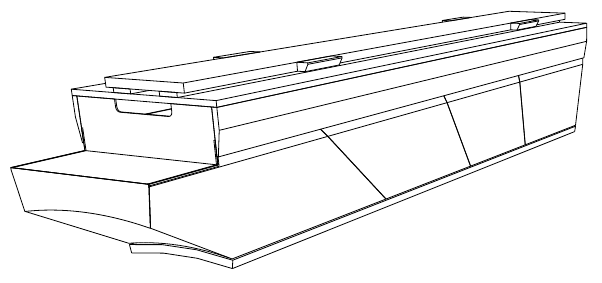
\includegraphics[width=0.6\textwidth]{figures/CMS/ECAL/cms_ecalSupermodule.png}
\caption{A view of the ECAL barrel supermodule which comprises four modules with 500 crystals in the first module and 400 crystals in each of the remaining three modules \cite{ECAL_TDR}.}
\label{fig:CMS_Ecal_Barrel_supermodule}
\end{center}
\end{figure}

The endcap part of the crystal calorimeter covers a pseudorapidity range from 1.48 to 3.0 (see Figure \ref{fig:CMS_Ecal_2}). The design of the endcaps provides precision energy measurement to $|\eta|$ = 2.6. However, the crystals will be installed up to $|\eta|$ = 3 in order to augment the energy-flow measurement in the forward direction. The mechanical design of the endcap calorimeter is based on an off-pointing pseudoprojective geometry using tapered crystals of the same shape and dimensions (24.7$\times$24.7$\times$220 $\mathrm{mm^{3}}$) grouped together into units of 36, referred to as supercrystals. A total of 268 identical supercrystals will be used to cover each endcap with a further 64 sectioned supercrystals used to complete the inner and outer perimeter. Each endcap contains 10764 crystals, corresponding to a volume of 1.52 \mThree (12.6 t). Both endcaps are identical and each endcap detector is constructed using Dee-shaped sections as seen Figure \ref{fig:CMS_Ecal_endcap}.

The endcap preshower covers a pseudorapidity range from $|\eta|$ = 1.65 to 2.61 (see Figure \ref{fig:CMS_Ecal_2}). Its main function is to provide \pizero-$\gamma$ separation. The preshower detector, placed in front of the crystals, contains two lead converters of a total thickness of 2$X_{0}$ and 1$X_{0}$ respectively, followed by detector planes of silicon strips with a pitch of $<$ 2 mm. The impact position of the electromagnetic shower is determined by the barycenter of the deposited energy and accuracy is typically 300 $\upmu$m at 50 GeV. In order to correct for the energy deposited in the lead converter, the energy measured in the silicon is used to apply corrections to the energy measurement in the crystal. The fraction of energy deposited in the preshower (typically 5\% at 20 GeV) decreases with increasing incident energy. Figure \ref{fig:CMS_Ecal_preshower} shows the layout of the preshower.

Figure \ref{fig:CMS_Ecal_3} shows the total thickness (in radiation lengths) of the ECAL as a function of
pseudorapidity where the endcap part also includes the preshower detector.




\begin{figure}[h!]
\begin{center}
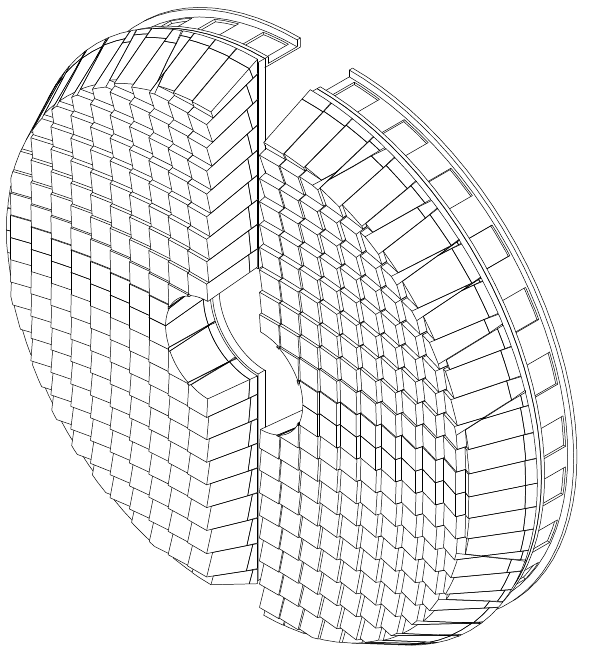
\includegraphics[width=0.5\textwidth]{figures/CMS/ECAL/cms_ecalEndcap.png}
\caption{A single endcap with Dee-shaped \cite{ECAL_TDR}.}
\label{fig:CMS_Ecal_endcap}
\end{center}
\end{figure}

\begin{figure}[h!]
\begin{center}
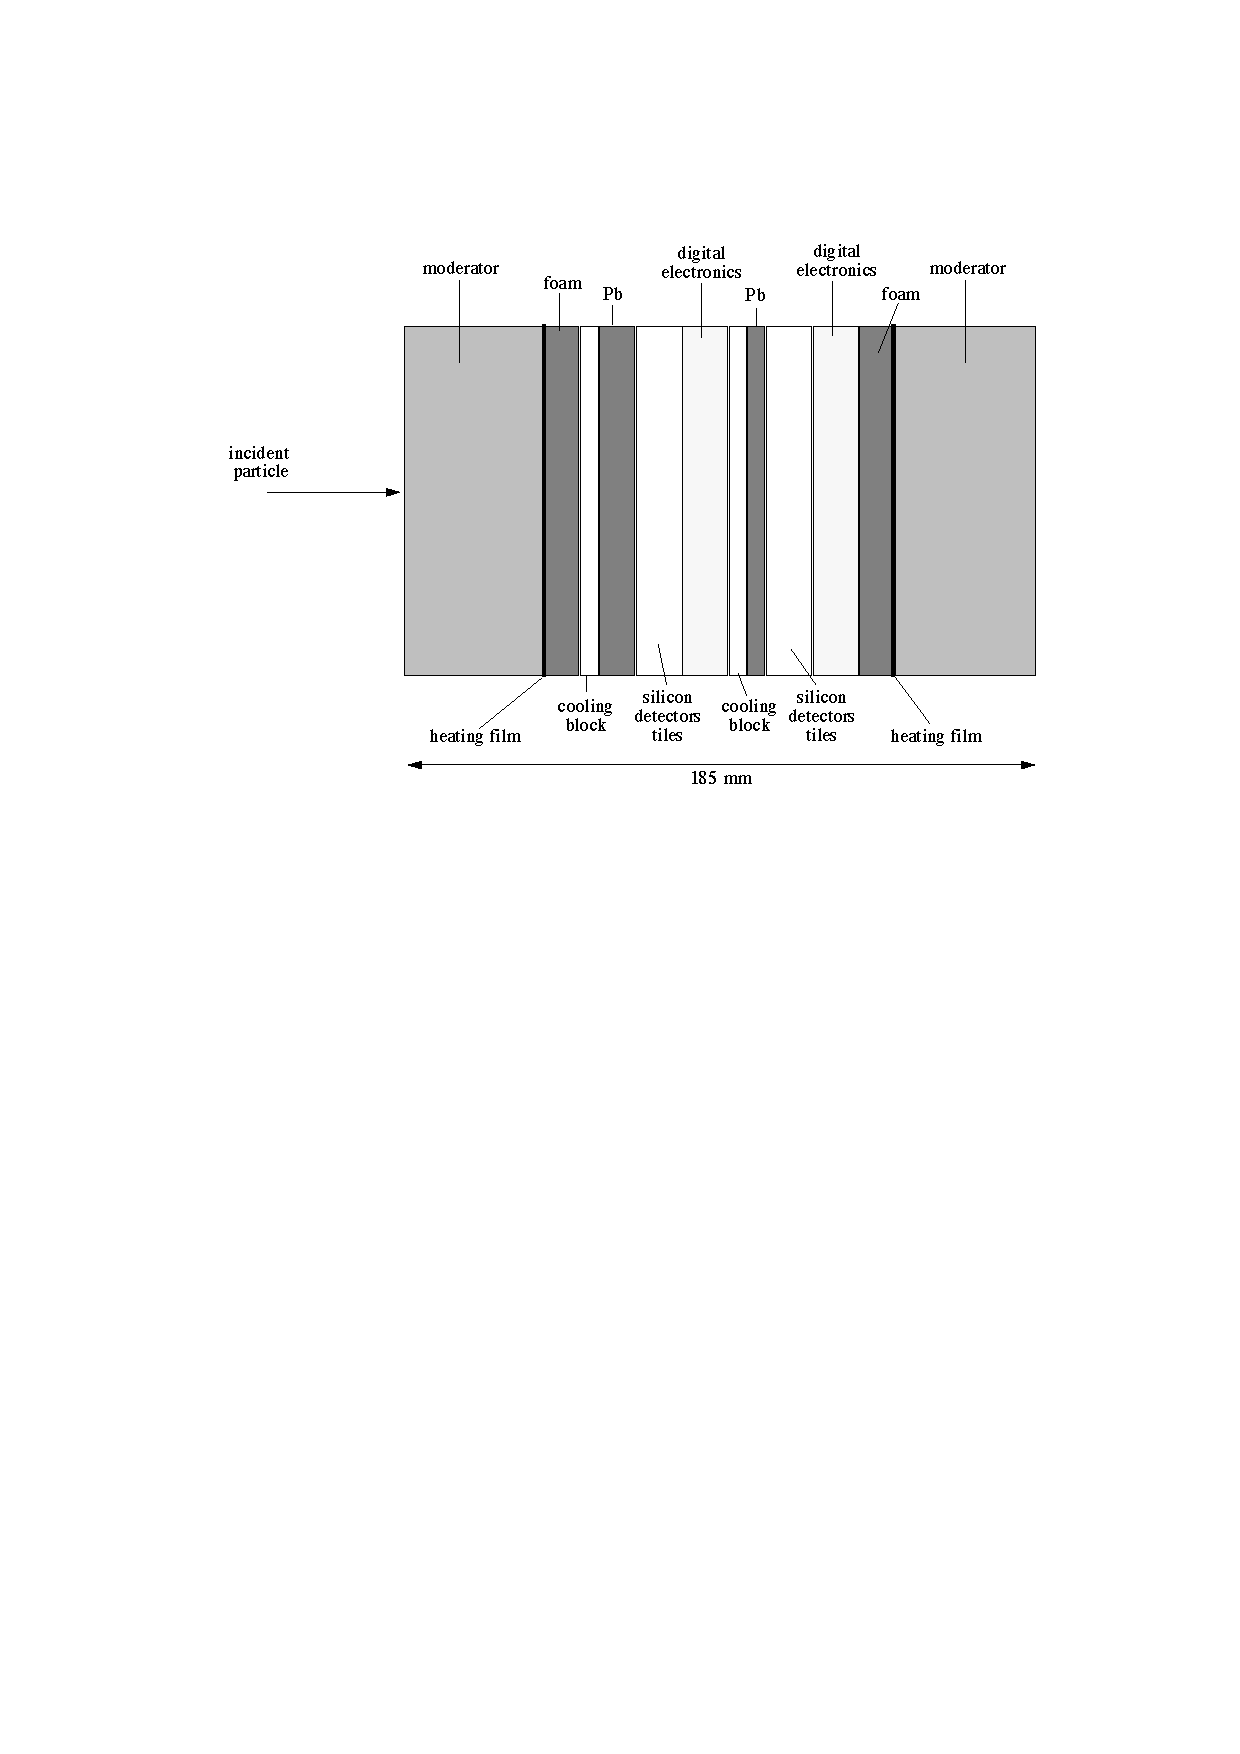
\includegraphics[width=0.8\textwidth]{figures/CMS/ECAL/ecalTDR/es-19.pdf}
\caption{The components of the endcap preshower \cite{ECAL_TDR}.}
\label{fig:CMS_Ecal_preshower}
\end{center}
\end{figure}


\begin{figure}[h!]
\begin{center}
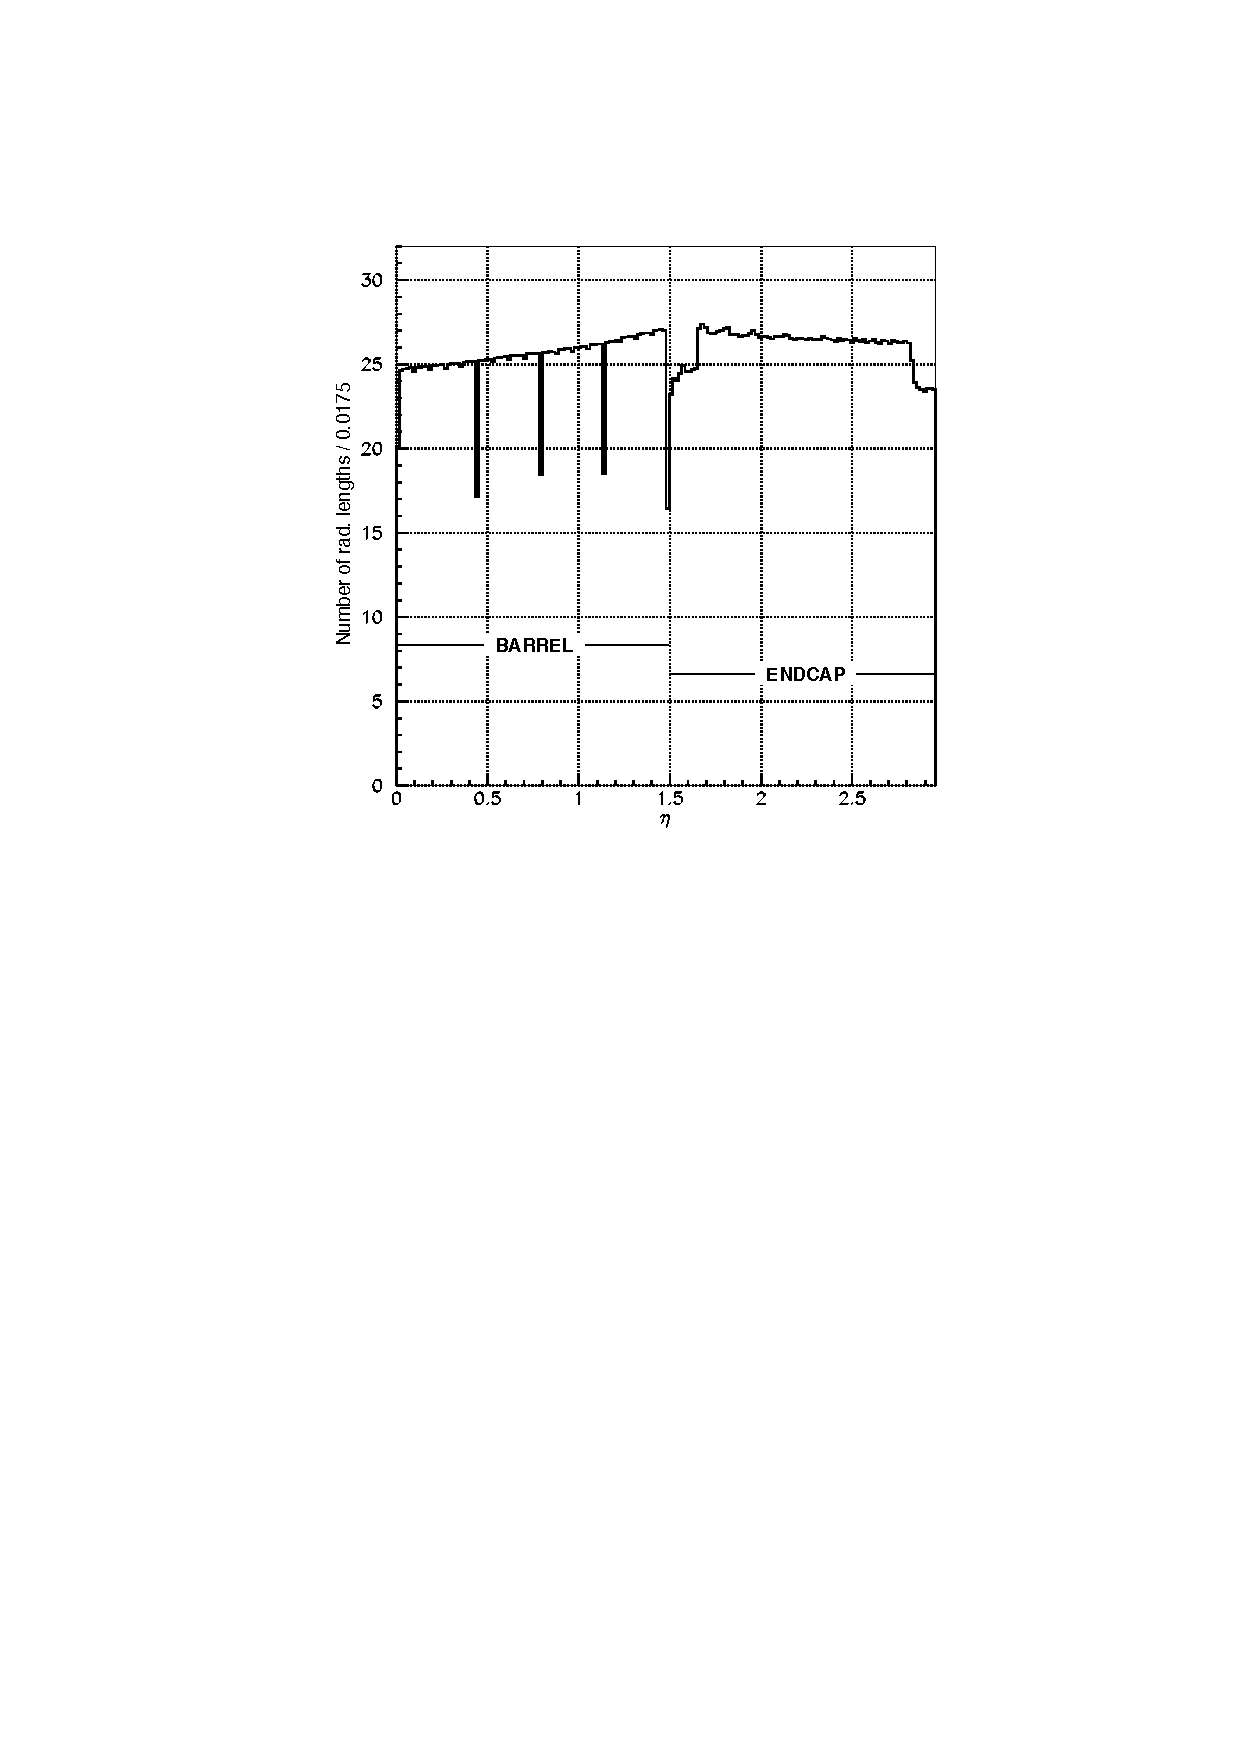
\includegraphics[width=0.6\textwidth]{figures/CMS/ECAL/ecalTDR/material-budget-17.pdf}
\caption{The thickness in $X_{0}$ of the ECAL as a function of pseudorapidity (averaged over $\phi$) \cite{ECAL_TDR}.}
\label{fig:CMS_Ecal_3}
\end{center}
\end{figure}

The energy resolution of the ECAL can be parameterized by the following expression \cite{ECAL_TDR}:

\begin{equation}
(\frac{\sigma}{E})^{2}=(\frac{S}{\sqrt{E}})^{2}+(\frac{N}{E})^{2}+C^{2}
\label{eq:ECAL_resolution}
\end{equation}

where $\sigma$ is the energy resolution, S is the stochastic term, N is the noise term, and C is the constant term. The stochastic term includes fluctuations in the shower containment as well as a contribution from photostatistics. The noise term contains the contributions from electronic noise and pile-up energy;
For instance, for 20 to 250 GeV of the electron test beam, with a 3$\times$3 crystal configuration, the measured value of the parameters is S = 0.028 $\sqrt{\mathrm{(GeV)}}$, N = 0.12 GeV, and C = 0.003.

%the former is quite important at low energy, the latter is negligible at low luminosity. The curve labeled \textit{intrinsic} in Figure \ref{fig:CMS_Ecal_resoultion} includes the shower containment and a constant term of 0.55\%.
%\begin{figure}[h!]
%\begin{center}
%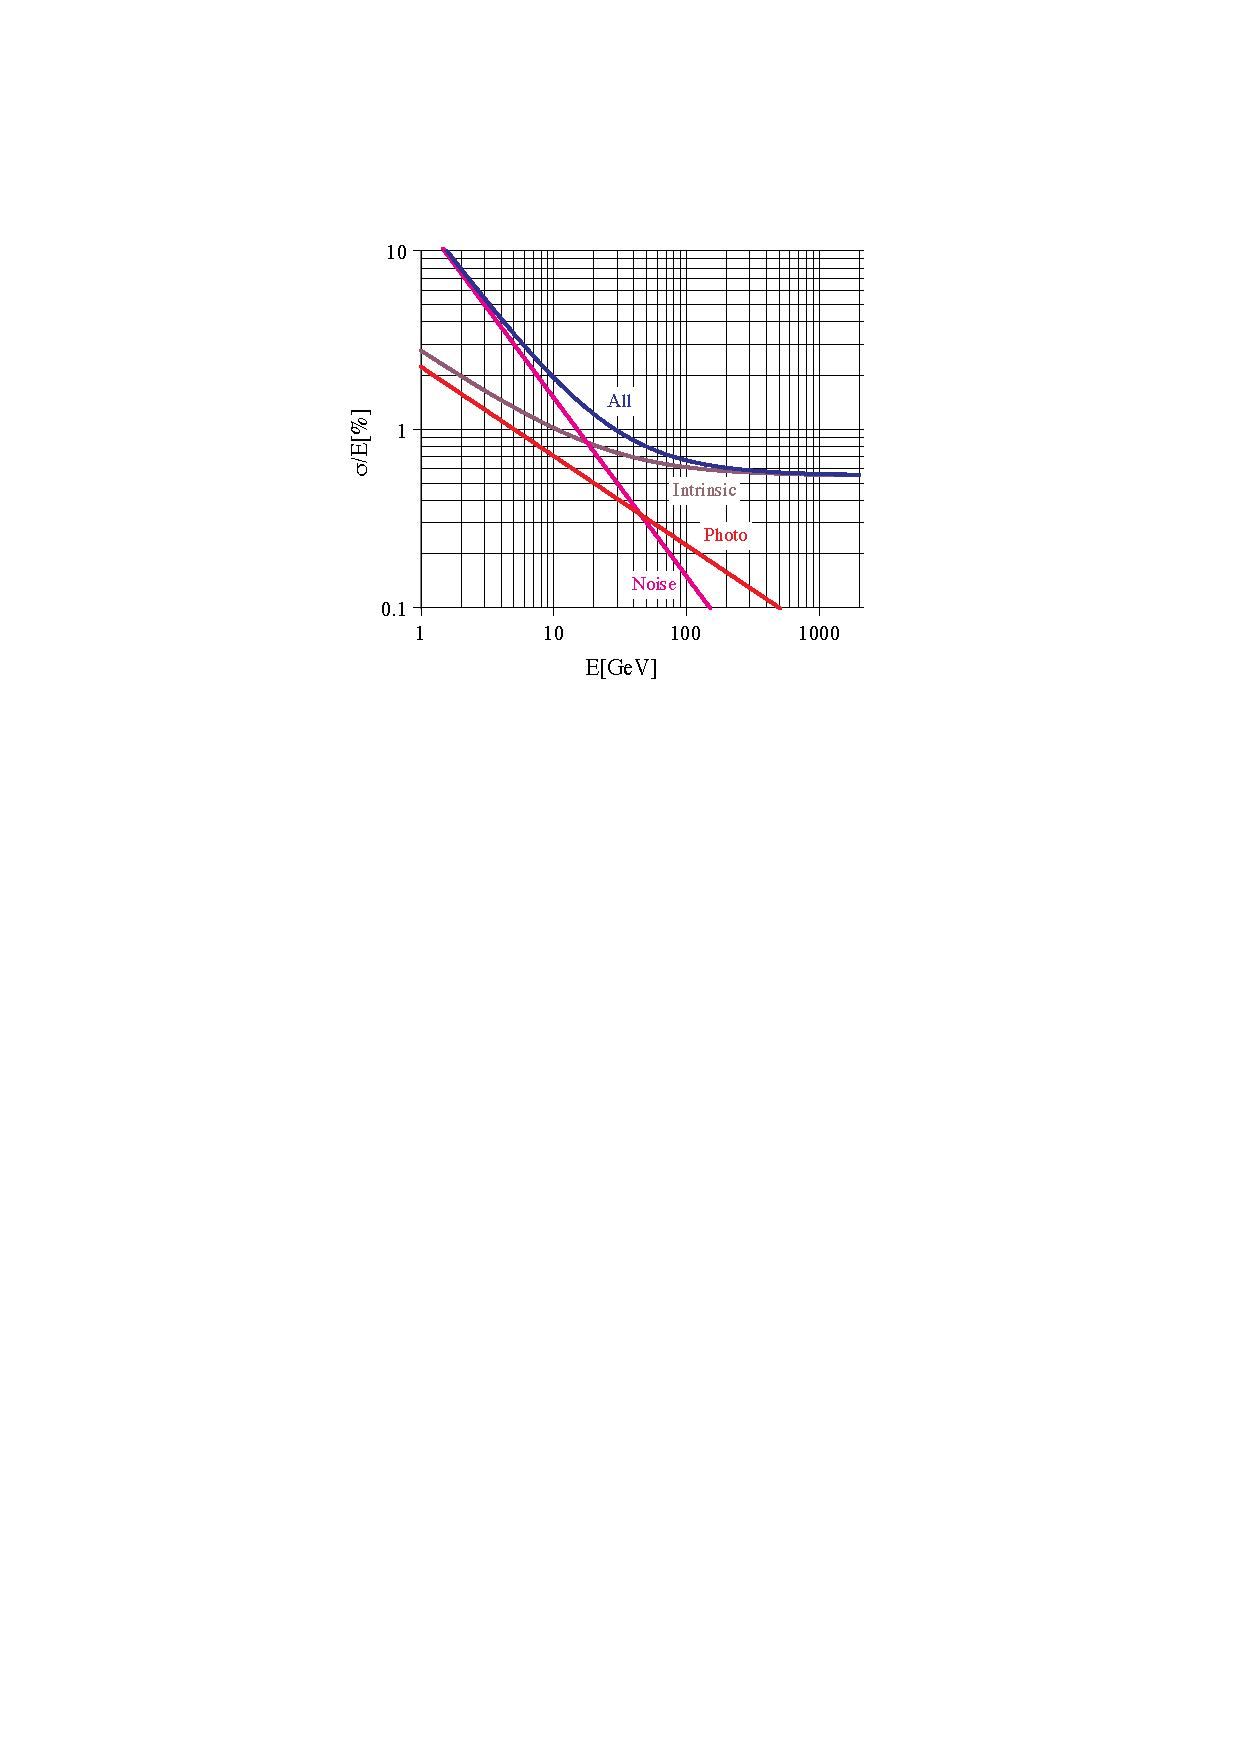
\includegraphics[width=0.8\textwidth]{figures/CMS/ECAL/ecalTDR/resolution-13.pdf}
%\caption{Different contributions to the energy resolution of the \PbWO calorimeter. The noise term contains the contributions from electronic noise and pile-up energy. The curve labelled  ``photo'' describes the contribution from photostatistics, while the curve labelled  ``intrinsic'' includes the shower containment and a costant term of 0.55\% \cite{ECAL_TDR}.}
%\label{fig:CMS_Ecal_resoultion}
%\end{center}
%\end{figure}


\subsection{Hadronic calorimeter}\label{subsec:CMS_HCAL}
In order to measure the energy of hadron (charged or neutral), CMS detector uses hadronic calorimeter (HCAL) which surrounds the ECAL system. The design of the HCAL is strongly influenced by the choice of the magnet parameters since most of the CMS calorimetry is located inside the magnet coil (see Figure \ref{fig:CMS_transversal}). An important requirement of HCAL is to minimize the non-Gaussian tails in the energy resolution and to provide good containment and hermeticity for the $\et^{miss}$ measurement (see Section \ref{sec:MET}). Hence, the HCAL design maximizes material inside the magnet coil in terms of interaction lengths. Brass has been chosen as absorber material as it has a reasonably short interaction length and is relatively easy to mold and it is non-magnetic.

The architecture of the HCAL is illustrated in Figure \ref{fig:CMS_HCAL}. The hadron barrel calorimeter (HB), located inside the magnet coil, covers pseudorapidity to 1.3 and is divided in $\eta\times\phi$ towers of dimension 0.087$\times$0.087. The HB is complemented by an additional layer of scintillators, referred to as the hadron outer (HO) detector which lining the outside of the magnet coil. The total thickness of the combination of the HB and the HO is around twelve interaction lengths. The hadron endcap calorimeter (HE) covers a pseudorapidity range 1.3 < $|\eta|$ < 3.0 and its thickness corresponds to approximately ten interaction lengths. Forward hadron calorimeters (HF) cover the high pseudorapidity regions (3.0 < $|\eta|$ < 5.2), as the particle flux in this very forward region is extremely high, a radiation hard technology, using Cherenkov light in quartz fibers was chosen and using steel as an absorber. The HF detector is also used as a real-time monitor for the luminosity on a bunch-by-bunch basis.
The overall assembly enables the HCAL to be built with essentially no uninstrumented cracks or dead areas in $\phi$. The gap between the HB and the HE, through which the services of the ECAL and the inner tracker pass, is inclined at $53^{\circ}$ and points away from the center of the detector.
The HCAL baseline single-particle energy resolution is \cite{CERN-LHCC-97-031}:

\begin{equation}
\frac{\sigma}{E}=\frac{X}{\sqrt{E}}\oplus5\%, \texttt{~X=65\% (in barrel), 83\% (in endcap), 100\% (in forward)}
\label{eq:HCAL_resolution}
\end{equation}




\begin{figure}[h!]
\begin{center}
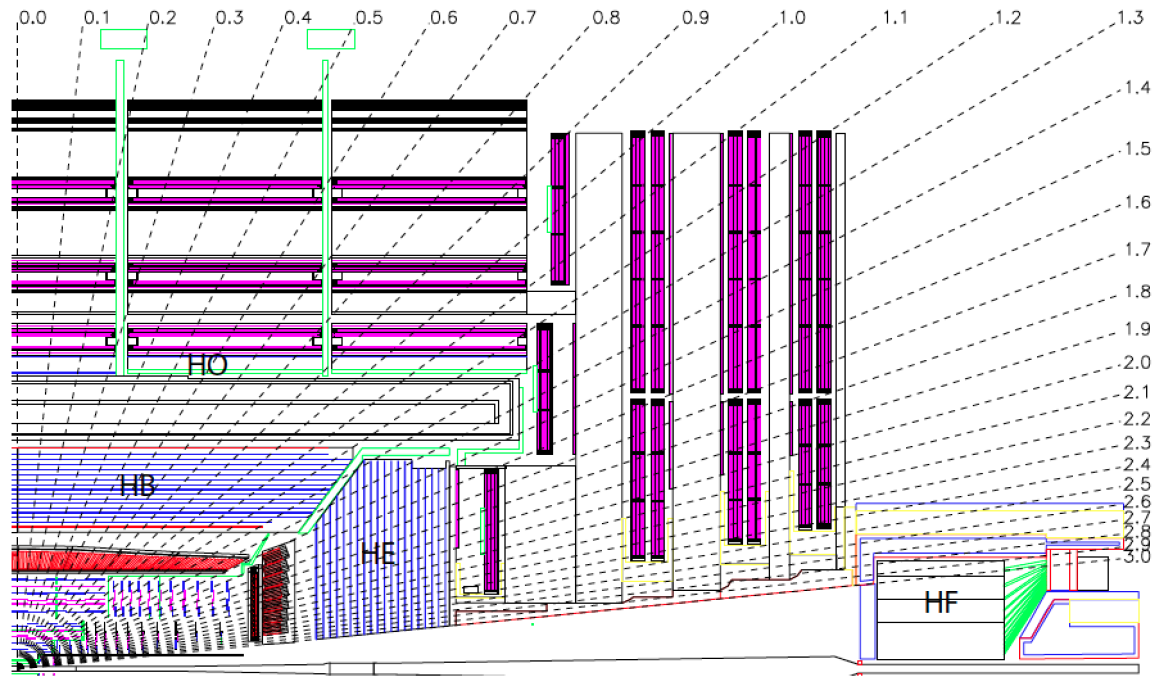
\includegraphics[width=0.8\textwidth]{figures/CMS/HCAL/HCAL.png}
\caption{Longitudinal view of the CMS detector. The locations of the hadron barrel (HB), endcap (HE), outer (HO), and forward (HF) calorimeters are indicated \cite{Chatrchyan:2008aa}.}
\label{fig:CMS_HCAL}
\end{center}
\end{figure}


\subsection{Magnet}\label{subsec:CMS_Magnet}
The CMS magnet is a superconducting solenoid magnet. Its length is 12.9 m and its inner diameter is 5.9 m. It can provide a 3.8 T strong magnetic field.
The magnet in CMS is used to bend the track of charged particle and the radius of the track in transverse plane can be used to measure the transverse momentum of the charged particle by
$$\mathrm{\pt=0.3R|Q|B}$$
where \pt (GeV) is the transverse momentum, R (m) is the radius of the track in transverse plane, $|\mathrm{Q}|$ (e) is the absolute charge of the particle (e.g. for electron it is 1) and B (T) is the magnetic field strength.
The design of the CMS magnet was driven by the required performance of the muon system (see next section). For example, for muon with momentum of 1 TeV, the $\Delta p/p$ should $\sim10\%$.

\subsection{Muon system}\label{subsec:CMS_muon}
The muon system is used to identify muons, to measure their momenta, and to contribute to the event triggering. It relies on three types of gaseous detectors, located outside the
magnet solenoid: drift tubes (DT), cathode strip chambers (CSC) and resistive plate chambers (RPC). The DT and the CSC provide an excellent spatial resolution for the measurement of charged particle momentum; the RPC are used for trigger issues because of its very fast time response. The active parts of the muon system are hosted into stations which are interleaved by the iron layers of the return yoke of the magnet. The longitudinal view of a quarter of the muon system is given in Figure \ref{fig:CMS_Muon}. The barrel of muon system (MB) is extended up to $|\eta|$<1.2, the endcap of muon system (ME) is for $1.2<|\eta|$ < 2.4.

\begin{figure}[h!]
\begin{center}
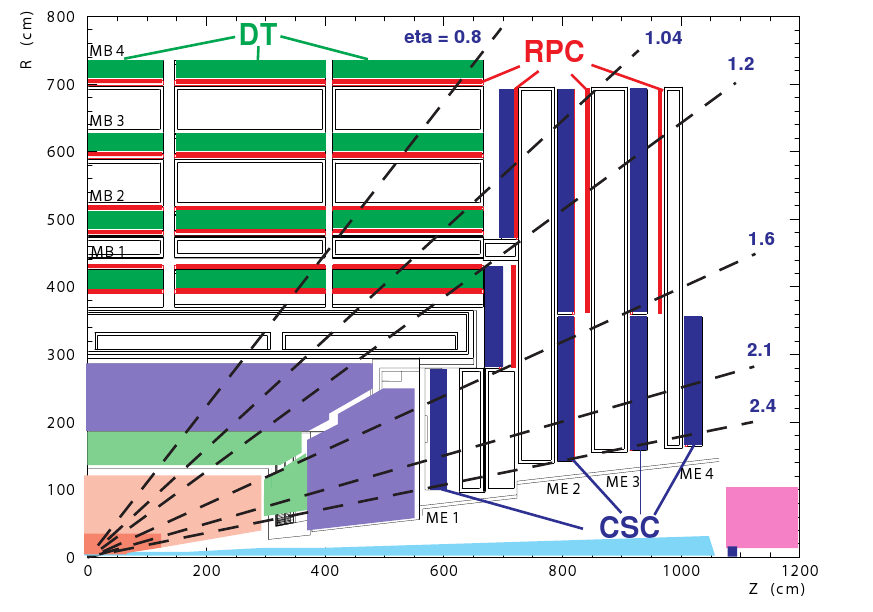
\includegraphics[width=0.8\textwidth]{figures/CMS/Muon/Muon.png}
\caption{Longitudinal view (one quarter) of the muon system \cite{Chatrchyan:2008aa}.}
\label{fig:CMS_Muon}
\end{center}
\end{figure}

In the MB there are four concentric muon stations (labeled MB1, MB2, MB3, and MB4 with the last being the outermost) consisting of 250 chambers inside the magnet return yoke. The MB is further divided into five wheels around the beam axis, which are themselves divided in twelve sectors, with each covering a $30^{\circ}$ azimuthal angle. The exact composition of the muon stations in terms of the number of DTs and their orientation, depends on the position of the station, and is chosen in such a way as to provide a good efficiency for reconstructing muon tracks from muon hits in different stations. The resolution of a single station is close to 100 $\upmu$m in position and 1 mrad in direction.

The ME comprises 468 CSCs in the 2 endcaps and is divided in four stations per endcap (labeled ME1, ME2, ME3, and ME4 with the last being the outermost). The CSCs, which consist in multiwire proportional chambers, have a trapezoidal shape and count six gas gaps, each gap having a plane of radial cathode strips and a plane of anode wires running almost perpendicularly to the strips. Unlike DT, they can support the high rate of neutron-induced background and cope with a large and non-uniform magnetic field. The spatial resolution provided by CSC is typically about 200 $\upmu$m and the angular resolution in $\phi$ is in the order of 10 mrad.

For low-momenta muons, the momentum resolution is by far dominated by the tracker measurements, while for particles with high momenta (around 1 TeV), the tracker and the muon system both provide a momentum resolution of about 5\%. Combining the inner tracker and the muon system, the transverse momentum resolution for particles up to 1 TeV lies between 1 and 5\%. Although DTs and CSCs can be used to trigger events based on the \pt of the muons with a good efficiency, their time response is comparable to the design bunch crossing space. Therefore, RPCs, which are double-gap chambers operated in avalanche mode, composed of parallel anode and cathode plates with a gas gap in between, have been introduced in the barrel and endcaps as a dedicated trigger system with a fast response and good time resolution. The position resolution of RPCs is however coarser than that of DTs and CSCs. Six layers of RPC are embedded in the barrel, whereas three layers of RPCs are in part of each endcap muon system.

Without complementary information form the tracker, the muon system provides a resolution of about 10\% for muons with $|\eta|$ < 2.4 and \pt < 200 GeV.

\subsection{Trigger}\label{subsec:CMS_trigger}

Because the proton bunch crossing frequency is 40 MHz at the CMS interaction point and the size of each collision event is around 1 MB, it is impossible to save all the events. Besides, most of the events from the collision are QCD events, which are less interesting for physics analysis. Therefore, the CMS developed a trigger system in order to save the events that are interesting for physics analysis. The trigger system is separated by to steps: Level-1 (L1) trigger and High-Level trigger (HLT).


The L1 triggers relies coarse information from calorimeters and the muon systems. Its decision is based on the \pt of specific objects like  e/$\gamma$, muons and jets. Due to the large time consuming of tracker reconstruction algorithm, the information from track system is not used in the L1. After applying the L1 trigger, the output event rate is around 100 kHz.

The event passing the L1 will then asked to pass the HLT. At the LHT stage, the information from track system will be used and the reconstructed objects at the HLT will be close to the one used in physics analysis. After applying the HLT, the finally total event rate is around few hundred hertz. If the event rate after the HLT is still very high for some specific trigger path, then a prescale value will be applied to that trigger path to reduce the event rate. Finally, all the information from the event passing the HLT will be transferred to mass storage and saved for physics analysis.


%Events passing the L1 Trigger are then processed by the HLT, which performs more complex calculations, based on a combination of information from the different subdetectors.
%The goal of the HLT is to reduce the event rate from the maximum L1 output ($\sim$100 kHz) to 600 Hz which is the maximum rate for mass storage. Once the L1 trigger has accepted
%an event, the data of this event are transferred from the buffer memory to the surface, where they are reconstructed in the HLT. The HLT is a special part of the CMS software
%and runs on a farm of several thousand processors. Each processor works on the reconstruction of one event at a time, to get to a trigger decision within 100 ms on average. Since the time budget for one event is much larger than at the L1 trigger, more complicated algorithms, including tracking, can be executed at the HLT level. Once an event is accepted, it is stored on disk and fully reconstructed offline at a later time. The HLT path starts from the seed of the L1 trigger which looks for different objects and signatures in the event. One trigger path is built from reconstruction modules and filter modules. After some parts of the data are reconstructed, a filter module decides either the reconstructed objects pass the thresholds and the next step in reconstruction is started, or the event is not accepted by the path. In the latter case, the execution of the path is stopped and the following reconstruction steps and filter steps are not performed to save computation time.
%
%If the acceptance rate from trigger is too high (for example in case of a trigger path with very low thresholds), the trigger path can be prescaled to lower the rate. For example, a prescale value 10 of HLT trigger means that the path is executed only for 1 over 10 events (randomly chosen to avoid biases) that were accepted by the L1 trigger and, consequently, the trigger rate for that HLT path is 10 times smaller. The prescale value for one trigger path has several predefined levels, depending on the instantaneous luminosity of the LHC machine. During an LHC fill, the instantaneous luminosity decreases, and the prescale values can be changed during a CMS run to keep the global trigger rate at an optimal level.

\section{Summary}\label{subsec:LHC_CMS_Summary}

In this chapter, a basic introduction about LHC is delivered including the main experiments at LHC, the LHC accelerator, the phenomenon of proton-proton collisions and pile up as well as the luminosity of LHC. After that a detailed description of the CMS detector is given which is composed of several subdetectors: the tracker system, the electromagnetic calorimeter, the hadronic calorimeter, the magnet, and the muon chambers.
